

\chapter{Mesures : Des S\'eries Temporelles}
\label{timeSeries}
Les mesures sur les arcs forment des s\'eries temporelles.
Certains arcs partagent des \'equipements que nous souhaitons d\'eterminer \`a partir des s\'eries temporelles. Nous supposons que les  s\'eries temporelles associ\'ees \`a ces arcs ont les m\^emes comportements au cours du temps. En d'autres termes, toute variation dans une s\'erie est visible dans une autre s\'erie. Nous disons que ces arcs sont {\em corr\'el\'es} et la valeur li\'ee \`a cette relation entre les arcs est d\'esign\'ee par {\em coefficient de similarit\'e}.  
\newline
Dans le chapitre pr\'ec\'edent, 
nous avons mod\'elis\'e les mesures sur les arcs par des s\'eries temporelles et la particularit\'e de ces s\'eries  est la pr\'esence de valeurs \'erron\'ees et manquantes. 
% quel est notre probleme
\newline
Le probl\`eme est de savoir s'il existe une m\'ethode de calcul du coefficient de similarit\'e qui tienne compte des erreurs dans les s\'eries temporelles et qui v\'erifie l'hypoth\`ese sous-jacente.
\newline
Pour ce faire, nous proc\'edons comme suit : la premi\`ere partie \'enonce  les analyses sur les s\'eries temporelles. La seconde partie pr\'esente les diff\'erentes m\'ethodes de calcul des coefficients de similarit\'e entre les s\'eries. Et enfin la derni\`ere partie s\'electionne la m\'ethode de calcul du {\em coefficient de similarit\'e} puis analyse les performances de cette m\'ethode sur les donn\'ees r\'eelles d'un {\em sous-r\'eseau du datacenter Champlan}.  

\section{S\'eries temporelles}
\begin{definition}
Une s\'erie temporelle est une suite chronologique de valeurs r\'eelles $x_t$ \`a des instants de temps r\'eguli\`erement espac\'es. 
% formule
\begin{equation}
(x_t)_{ t \in \Theta}
\end{equation}
avec $\Theta $ l'ensemble discret et fini des espaces de temps de dimension $n$.
\end{definition}
L'intervalle de temps entre deux mesures successives d\'epend de la s\'erie. 
Il peut s'agir d'une minute, d'une semaine, d'un jour, etc.
%G\'en\'eralement, les s\'eries temporelles s'utilisent dans les probl\`emes suivants :
G\'en\'eralement, les s\'eries temporelles sont utilis\'ees  pour comprendre les m\'ecanismes qui produisent ces observations. Ces m\'ecanismes sont associ\'es au temps et  permettent de faire les analyses suivantes :
\begin{itemize}
	\item La mod\'elisation : la repr\'esentation de la s\'erie sous la forme d'une fonction du temps.
	\item La pr\'evision : pr\'edire les donn\'ees futures \`a partir de valeurs pr\'ed\'ecentes.
	\item La d\'etection de rupture :  la s\'erie change-t-elle significativement \`a un instant $t$.
	\item La comparaison :  d\'eterminer la relation existante entre une s\'erie observ\'ee et d'autres s\'eries candidates.
\end{itemize}
Nous d\'ecrivons bri\`evement les mod\`eles d'analyses sur des s\'eries temporelles puis nous pr\'esentons l'objectif recherch\'e par l'analyse de ces s\'eries dans notre \'etude. 

\subsection{La mod\'elisation et la pr\'evison d'une s\'erie temporelle}
Un mod\`ele est une image simplifi\'ee de la r\'ealit\'e qui vise \`a traduire le fonctionnement d'un ph\'enom\`ene et permet de mieux les comprendre.
Nous distinguons deux types de mod\`eles :
\begin{itemize}
	\item Les mod\`eles d\'eterministes : ils utilisent les \'el\'ements de la statistique descriptive et suppose que l'observation de la s\'erie \`a la date $t$ est une fonction du temps $t$ et d'une variable $\epsilon_t$: 
	$$x_t = f(t, \epsilon_{t}).$$ 
	La variable $\epsilon_t$ est le r\'esidu ou l'erreur du mod\`ele et elle repr\'esente la diff\'erence entre la r\'ealit\'e et le mod\`ele propos\'e. 
	\newline
	Les deux mod\`eles les plus utilis\'es sont les suivants :
	\begin{itemize}
		\item Le mod\`ele additif : c'est la d\'ecomposition de la s\'erie en trois termes
			$$x_t = Z_t + S_t + Q_t $$ o\`u $Z_t$ est la tendance, $S_t$ la p\'eriodicit\'e et $Q_t$ les composantes (erreurs) identiquement distribu\'ees. $Z_t$, $S_t$ sont aussi d\'eterministes.
		\item Le mod\`ele multiplicatif : la variable $x_t$  est le produit de la tendance et d'une composante p\'eriodique :
		$$x_t = Z_t(1 + S_t)(1 + Q_t).$$
		Toutefois, l'application d'un logarithme nous permet de revenir au mod\`ele additif.
		$$y(t) = log(x_t) = log(Z_t) +log(1 + S_t) + log(1 + Q_t).$$
	\end{itemize}
	%L'utilisation de mod\`eles d\'eterministes pour la pr\'evision est \'el\'ementaire. Une fois d\'etermin\'ee la fonction $f$ \`a partir des donn\'ees observ\'ees $x_1 , ... , x_n$ , nous proposons une pr\'evision \`a la prochaine date par $\hat{X_{n+1}} = f(n+1)$.La pr\'ecision de cette pr\'evision peut aussi \^etre \'evalu\'ee par une estimation de la variance de $\epsilon_{n+1} = \hat{X_{n+1}} - f(n+1)$ . Cette estimation est r\'ealis\'ee par la variance empirique de la s\'erie des \'ecarts $\epsilon_i = X_{i} - f(i)$, consid\`er\'ee comme une s\'erie de variables al\'eatoires ind\'ependantes de m\^eme loi. La donn\'ee de cette variance empirique permettra de proposer un intervalle de confiance autour de la pr\'evision.

	\item Les mod\`eles stochastiques : ils font l'hypoth\`ese que les r\'esidus $\epsilon_t$ ne sont pas ind\'ependants et qu'il est possible de pr\'evoir les r\'esidus en partie. L'avantage r\'eside dans la r\'eduction de l'impr\'ecision de la pr\'evision des termes futurs de la s\'erie temporelle.  La variable $\epsilon_t$ devient une fonction des valeurs du pass\'e et d'un terme d'erreur $\eta_t$ $$\epsilon_t = (\epsilon_{t-1}, \epsilon_{t-2}, ... , \eta_{t}).$$
	Nous pouvons citer, comme exemple de mod\`eles couramment utilis\'es, les mod\`eles SARIMA, ARIMA et ARMA. Dans ces mod\`eles, la mod\'elisation porte sur la forme du processus $(\epsilon_t)$. Un exemple de mod\'elisation est le mod\`ele autor\'egressif lin\'eaire d'ordre $2$ avec des coefficients autor\'egressifs $a_1$, $a_2$ d\'efinis par 
	$$\epsilon_t = a_1 x_{t-1} + a_2 x_{t-2} + \eta_t,$$ o\`u $\eta_t$ est un bruit blanc.
\end{itemize}
Un exemple de s\'erie temporelle et de ses diff\'erentes composantes est pr\'esent\'e dans la figure \ref{exempleSerieTemporelleComposante}. La s\'erie temporelle est la donn\'ee du trafic prise chaque mois des routes fran\c caises de $1989$ \`a $1996$.
La premi\`ere ligne est la r\'epresentation de la s\'erie temporelle et la seconde est celle de la tendance. Quant \`a la troisi\`eme  et la derni\`ere ligne, elles repr\'esentent respectivement la figure de p\'eriodicit\'e et les r\'esidus. La p\'eriode de la s\'erie est de $12$.
% ---- figure exemple de la serie temporelle et ses composante
\begin{figure}[htb!] 
\centering
\includegraphics[scale = 0.5]{exempleSerieTemporelleComposante.pdf}
%\includegraphics[scale = 0.5]{/home/willy/Downloads/exempleSerieTemporelleComposante.pdf}
\caption{ 
	D\'ecomposition de la s\'erie temporelle representant les valeurs mensuelles du trafic routier de l'autoroute $A7$ de $09/1989$ \`a $09/1996$. Repr\'esentation des composantes de la s\'erie temporelle.} 
\label{exempleSerieTemporelleComposante}
\end{figure}
%\FloatBarrier
% ---- figure exemple de la serie temporelle et ses composante

Les deux types de mod\`eles ci-dessus induisent des techniques de pr\'evision bien particuli\`eres. 
Sch\'ema--tiquement, ils s\'eparent la tendance de la saisonnalit\'e \'eventuelle. Puis ils cherchent \`a les mod\'eliser et \`a les estimer.  Enfin ils les \'eliminent de la s\'erie : ces deux op\'erations sont nomm\'ees
la {\em d\'etendancialisation} et la {\em d\'esaisonnalisation} de la s\'erie. Une fois ces composantes \'elimin\'ees, on obtient la s\'erie al\'eatoire $\epsilon_t$ :
%\vspace{-0.2cm}
\begin{itemize}
	\item Pour les mod\`eles d\'eterministes, cette s\'erie est consid\'er\'ee comme d\'ecorr\'el\'ee et il n'y a plus rien \`a faire.
	\item Pour les mod\`eles stochastiques, on obtient une s\'erie stationnaire (ce qui signifie que les observations successives de la s\'erie sont identiquement distribu\'ees mais pas n\'ecessairement ind\'ependantes) qu'il s'agit de mod\'eliser.
\end{itemize}
%L'utilit\'e de la mod\'elisation de s\'eries temporelles est couramment utilis\'e dans les 

\subsection{La d\'etection de rupture}
La d\'etection de rupture consiste \`a d\'eceler la pr\'esence d'un ou de plusieurs pics dans la s\'erie temporelle et \`a les localiser dans la s\'erie temporelle. 
D\'eterminer l'existence d'une rupture est d'autant plus difficile que cette derni\`ere n'est pas forc\'ement caract\'eris\'ee par un d\'ecalage de grande amplitude entre $x_t$ et $x_{t+1}$ par rapport \`a la dispersion des observations. 
Un enjeu de la d\'etection est donc d'\^etre sensible aux faibles variations tout en garantissant une certaine robustesse au bruit.
La th\`ese de master de {\em Flore Harl\'e} \cite{floreHarleDetectionRuptureMultiples2006} 
propose une m\'ethode de d\'etection de changements univari\'ee et multivari\'ee \`a la m\'ediane des segments, le segment \'etant une subdivision de la s\'erie temporelle. Les mod\`eles propos\'es sont exprim\'es par des fonctions de vraisemblance afin d'illustrer l'augmentation de la difficult\'e lors de l'ajout de nouvelles inconnues.

\subsection{La comparaison de  s\'eries temporelles}
Si deux s\'eries sont observ\'ees, nous pouvons nous demander quelle influence elles exercent l'une sur l'autre. 
Par exemple, \'etant donn\'ee deux s\'eries $X_t$ et $Y_t$, nous v\'erifions s'il existe par exemple des relations du type
$Y_t = a_1 \times X_{t+1} + a_3 \times X_{t+3}. $
\newline
Ici, deux questions se posent : tout d'abord, la question de la causalit\'e c'est-\`a-dire quelle variable (ici ($X_t$)) va expliquer l'autre (ici ($Y_t)$), ce qui conduit \`a la deuxi\`eme question, celle du d\'ecalage temporel: si une influence de $(X_t)$ sur $(Y_t)$ existe, avec quel d\'elai et pendant combien de temps la variable explicative $(X_t)$ influence-t-elle la variable expliqu\'ee $(Y_t)$ ?
\newline

%Dans notre cas d'\'etude, nous cherchons \`a comparer des s\'eries temporelles en supposant que les variation dans une s\'erie sont observables dans une autre s\'erie
%Ainsi, deux s\'eries $x_1$ et $x_2$ sont identiques s'il existe une s\'erie $k(t)$ de moyenne constante $K$ et d'\'ecart-type nul $\sigma_k = 0$ telle que 
%$$ \forall t \in \Theta, x_1(t) = k(t) \times x_2(t) .$$
Nous allons consid\'erer un r\'eseau de flots mod\'elis\'e par un graphe $G$ et les arcs portent des mesures. Les mesures sont mod\'elis\'ees par des s\'eries temporelles.
Dans notre cas d'\'etude, nous cherchons \`a comparer des s\'eries temporelles en supposant que les variations dans une s\'erie sont observables dans une autre s\'erie. Pour ce faire, nous rappelons que le coefficient de similarit\'e est une valeur indiquant la relation existante entre deux arcs et nous d\'efinissons la corr\'elation entre des arcs comme suit : 

\begin{definition}  Corr\'elation entre arcs\newline
Soit $corr$ le coefficient de similarit\'e entre les s\'eries $x$ et $y$ d\'efini de $\mathbb{R}^{n} \times \mathbb{R}^{n}
 \rightarrow [0,1]$ et 
 les arcs $A$ et $B$ contenant respectivement les s\'eries $x$ et $y$.
 \newline
Deux arcs $A$ et $B$ sont corr\'el\'es si et seulement si le coefficient de similarit\'e entre les s\'eries $x$ et $y$ est contenu dans $[0.5,1]$. 
($corr(x, y) \in [0.5,1]$)
\end{definition}
On dit alors que  $A$ et $B$ sont {\em fortement  corr\'el\'es} si 
le coefficient de similarit\'e est contenu dans l'intervalle $[0.7, 1]$ ($corr(x, y) \in [0.7,1]$) et {\em faiblement corr\'el\'es} si $corr(x, y)$ appartient \`a l'intervalle $[0.5,0.7[$ ($corr(x,y) \in [0.5, 0.7[$).
\newline




Notre objectif est de trouver la m\'ethode qui calcule au mieux la corr\'elation entre des arcs en tenant compte des caract\'eristiques de nos donn\'ees (valeurs manquantes et erron\'ees \`a certains instants $t$ dans les s\'eries temporelles des arcs).


\section{\'Etat de l'art des m\'ethodes de similarit\'e}
Les diff\'erentes m\'ethodes de calculs des coefficients de similarit\'e se basent sur les s\'eries temporelles associ\'ees aux arcs du r\'eseau.
Nous allons pr\'esenter les principales m\'ethodes de calculs de similarit\'e qui sont regroup\'ees en $3$ familles et qui sont d\'etaill\'ees dans cette section.
\subsection{ Similarit\'e sur les s\'eries enti\`eres}
	\label{seriesEntieres}
	Les s\'eries enti\`eres sont consid\'er\'ees comme des vecteurs et compar\'ees avec une distance qui utilise toutes les valeurs des s\'eries. 
%L'utilisation de toutes les valeurs est exig\'ee parce que les valeurs de chaque s\'erie peuvent \^etre diff\'erente \`a n'importe quel temps.
Cette distance calcule la similarit\'e entre ces deux s\'eries.
La similarit\'e entre deux s\'eries enti\`eres est excellente  s'il existe des caract\'eristiques discriminatoires identiques entre ces s\'eries sur l'axe du temps. Ces caract\'eristiques peuvent \^etre identifi\'ees aux m\^emes instants de temps ou \`a des instants d\'ecal\'es mais constants dans le temps. 
\newline
Par exemple, consid\'erons le dataset {\em FiftyWord} \cite{rath2003word} dans lequel les donn\'ees proviennent de la base de donn\'ee {UCR} \cite{chen2015ucr} et d\'ecrivent les contours des mots \'ecris par Georges Washington dans sa biblioth\`eque priv\'ee. Dans la figure \ref{caracteristiquesFiftyWordUCR}, nous distinguons $4$ s\'eries regroup\'ees en $2$ classes. Les deux s\'eries du haut (en noir) identifient la classe $30$ et les deux s\'eries du bas (en vert) identifient la classe $50$. Le motif commun est observable en alignant les s\'eries.
% ---- figure caracteristiquesFiftyWordUCR.
\begin{figure}[htb!] 
\centering
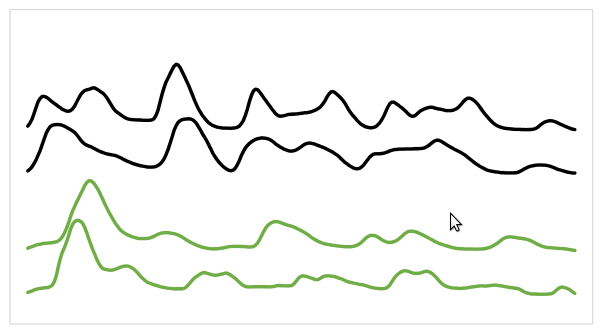
\includegraphics[scale = 0.5]{caracteristiquesFiftyWordUCR.jpeg}
\caption{D\'etection du motif commun en alignant les s\'eries. Les deux s\'eries du haut repr\'esentent la classe $30$ et les deux s\'eries du bas repr\'esentent la classe $50$.}
\label{caracteristiquesFiftyWordUCR}
\end{figure}
% ---- figure caracteristiquesFiftyWordUCR.

Les approches bas\'ees sur les vecteurs sont pertinentes quand il existe un d\'ecalage de temps entre les pics et les creux des s\'eries, comme c'est le cas avec les deux courbes du bas dans la figure \ref{caracteristiquesFiftyWordUCR}. 
\newline
Les m\'ethodes telles que 
{\em Time Warp Edit}, {\em Move-Split-Merge}, 
%{\em Elastic Ensemble}, {\em Collective Of Transform Ensemble} 
{\em Longest Common Subsequence } et 
{\em distance de Pearson} sont des distances de {\em mesures \'elastiques} qui se servent de l'approche vectorielle. 
Les  distances de {\em mesures \'elastiques} sont les meilleures approches pour traiter les probl\`emes des s\'eries enti\`eres \`a savoir la d\'etection de pics, de d\'ecalage et de creux entre les s\'eries.


	\subsubsection{Dynamic Time Warping  DTW}
		% ---- figure DTW
\begin{figure}[htb!] 
\centering
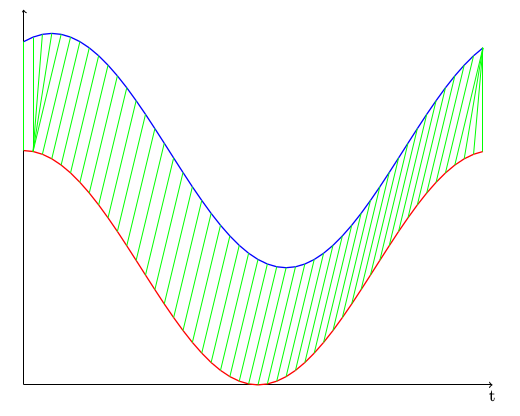
\includegraphics[scale = 0.5]{DTW2courbes.png}
\caption{Deux s\'equences en dimension $1$ align\'ees avec Dynamic Time Warping. Les coordonn\'ees de la s\'equence du haut et de celle du bas correspondent respectivement \`a
$cos(t)$ et \`a $cos(t+\alpha)$. 
Pour des questions de visualisation, la s\'equence du dessus a \'et\'e d\'ecal\'ee vers le haut lors du trac\'e. \cite{petitjean2011descriptionDTWexemple}
}
\label{DTW2courbes}
\end{figure}
% ---- figure DTW.

{\em Dynamic time warping (DTW) } est une technique pour trouver l'aligmenent optimal entre deux s\'equences d\'ependant du temps sous certaines contraintes (figure \ref{DTW2courbes}). 
Les s\'eries temporelles sont d\'eform\'ees par une transformation non-lin\'eaire de la variable temporelle, pour d\'eterminer une mesure de leur similarit\'e, ind\'ependamment de certaines transformations non-lin\'eaires du temps.
\newline
Supposons que nous souhaitons mesurer la similarit\'e entre deux s\'eries $A = (a_1, \cdots, a_m)$ et $B = (b_1, \cdots, b_m)$.
Soit $M(A,B)$ la matrice de distances entre $A$ et $B$ o\`u $M_{i,j} = (a_i - b_j)^2$.
Un chemin d'alignement {\em Dynamic Time Warping (DTW)} est une m\'ethode inspir\'ee de la distance de {\em Levenshtein}, \'egalement appel\'e {\em distance d'\'edition}. \`A l'origine, {\em DTW} \'etait appliqu\'e  dans le domaine de la reconnaissance vocale et permet de trouver l'alignement global optimal entre deux s\'equences, c'est-\`a-dire faire correspondre chaque \'el\'ement de chaque s\'equence \`a au moins un \'el\'ement de l'autre s\'equence en minimisant les co\^uts d'association. 
Le co\^ut d'une association correspond \`a la distance entre les deux \'el\'ements; classiquement une $l_p$ norm \cite{chen2004marriageLpNorm}.
La figure \ref{DTW2courbes} repr\'esente un exemple d'alignement op\'er\'e par {\em DTW}.
Il illuste l'alignement de deux sinusoides l\'eg\`erement d\'ephas\'ees. Le r\'esultat num\'erique fournit par {\em DTW} correspond \`a la somme des hauteurs des ``barreaux'' form\'es par les associations. Les extr\'emit\'es des alignements de la figure \ref{DTW2courbes} montrent que {\em DTW} est capable de r\'ealigner correctement une s\'equence par rapport \`a une autre, et parvient ainsi \`a saisir des similarit\'es que la
distance euclidienne ne peut extraire.
\newline
La distance {\em Dynamic Time Warping} est d\'efinie r\'ecursivement par :
$$
D(A_i, B_j) = \delta(A_i,B_j) + min
				\begin{cases}
				D( A_{i-1}, B_{j-1}), \\
				D( A_{i}, B_{j-1}), \\
				D( A_{i-1}, B_{j}))
				\end{cases}
$$
o\`u $A_i$ repr\'esente la sous-s\'equence $(a_1, \cdots, a_i)$. 
Le co\^ut de l'alignement optimal est alors donn\'e par
$ D(A_{|A|}, B_{|B|})$.
Le principe de programmation dynamique peut alors se r\'esoudre par un arbre en partant des
feuilles en supposant que le probl\`eme principal peut \^etre symbolis\'e par la racine et les sous-probl\`emes par des noeuds appartenant aux diff\'erents sous-arbres.
La fonction DTW peut alors \^etre m\'emois\'ee : les diff\'erents appels peuvent \^etre retenus afin de ne pas calculer deux fois la fonction appel\'ee avec les m\^emes param\`etres. 
Aussi est-il habituel, comme l'arbre contient
$| A | . | B |$ noeuds diff\'erents, de stocker ces diff\'erents r\'esultats interm\'ediaires dans une matrice $|A| \times | B |$.
Le calcul de $DTW$ consiste alors \`a trouver le chemin de co\^ut minimum dans la matrice, ce qui s'ex\'ecute avec une complexit\'e en temps et en m\'emoire de $\Theta(|A| \times |B|)$.

	\subsubsection{Time Warp Edit TWE}
		La distance {\em Time Warp Edit} (TWE) est une mesure de distance pour des s\'eries temporelles  discr\`etes. En comparaison avec les distances telles {\em Dynamic Time Warping (DTW)} \cite{muller2007dynamicDTW} et {\em longest common subsequence (LCS)} \cite{greenberg2002fastLCS}, la distance {\em TWE} est une m\'etrique propos\'ee par {\em P.F. Marteau} en $2009$. 
La distance {\em TWE} a quatre propri\'et\'es :
\begin{itemize}
	\item Traite le d\'ecalage temporelle local avec des performances \'elev\'ees.
	\item Satisfait l'in\'egalit\'e triangulaire c'est-\`a-dire $AB \le AC+CB$ avec $AB,AC, CB$ des cot\'es d'un triangle quelconque.
	\item Comprend le param\`etre de rigidit\'e $\nu$ qui contr\^ole l'\'elasticit\'e de la m\'etrique.
	\item Utilise la diff\'erence de temps pour comparer les segments de s\'eries temporelles comme des co\^uts de correspondances locales. 
\end{itemize}
Le param\`etre $\nu$ est important dans l'algorithme de {\em TWE} parce qu'il rend plus flexible l'identification de motifs (matching) entre les s\'eries temporelles. 
La preuve de son efficacit\'e a \'et\'e prouv\'ee dans \cite{marteau2009time}.

L'algorithme de {\em TWE} introduit trois op\'erations : $delete_A$, $delete_B$ et $match$ pour l'\'edition de deux s\'eries discr\`etes $A$ et $B$. L'\'edition d'une s\'erie temporelle consiste \`a modifier cette s\'erie en sous-ensembles de m\^emes tailles \`a partir d'une des trois op\'erations et chaque sous-ensemble est d\'esign\'e par  {\em s\'equence}. La similarit\'e entre les s\'eries $A$ et $B$ est le co\^ut minimum de s\'equences n\'ecessaire pour transformer $A$ en $B$.
En se basant sur ces trois op\'erations, l'algorithme de {\em TWE} calcule le co\^ut d'une s\'equence \`a chaque op\'eration pour toutes les paires de s\'eries avec l'\'equation \ref{coutSequenceTWE}. Dans cette \'equation, $U$ d\'esigne l'ensemble des s\'eries finies $U = \{A_1^p ~|~ p\in \N \}$ o\`u $A_1^p$ est une s\'erie avec des temps discrets variant de $1$ \`a $p$,
 $A_1^0$ est la s\'erie nulle de longueur nulle et 
 $a'_i$ d\'esigne le $i^{ieme}$ \'el\'ement de la s\'erie $A$.
Nous consid\'erons alors que $a'_i \in S \times T$ o\`u $S \subset R^d$ avec $d \ge 1$ int\`egre un espace multidimensionnel de variables et $T \subset R$  int\`egre la variable temporelle.
Ainsi, nous pouvons \'ecrire $a'_i = (a_i, t_{a_i})$, o\`u $a_i \in S$ et $t_{a_i} \in T$ avec la condition que  $t_{a_i} > t_{a_j}$ quand $i > j$ (le temps est strictement croissant dans la s\'equence des \'el\'ements).
La p\'enalit\'e not\'ee $\lambda$ est constante.
La similarit\'e entre les s\'eries $A$ et $B$ est calcul\'ee r\'ecursivement par 
\begin{equation}
	\delta_{\lambda,\nu}(A_1^p, B_1^q) = min
	\begin{cases}
		\delta_{\lambda,\nu}(A_1^{p-1}, B_1^q) + \Gamma(a'_p \rightarrow \Lambda) ~~~~~ delete_A, \\
		 \delta_{\lambda,\nu}(A_1^{p-1}, B_1^{q-1}) + \Gamma(a'_p \rightarrow b'_q) ~~~~~ match, \\
		 \delta_{\lambda,\nu}(A_1^{p-1}, B_1^q) + \Gamma(\Lambda \rightarrow a'_p) ~~~~~ delete_B, \\
	\end{cases}
	\label{coutSequenceTWE}
\end{equation} 
avec 
 \[
	\begin{array}{lcl} 
	\Gamma(a'_p \rightarrow \Lambda) & = & d(a'_p, a_{p-1}) + \lambda  \\ 
	\Gamma(a'_p \rightarrow b'_q) & = & d(a'_p, b'_{q}) + d(a'_{p-1}, b'_{q-1}) \\
	\Gamma(\lambda \rightarrow b'_q)  & = & d(b'_q, b'_{q-1}) + \lambda. 
	\end{array}
\]
La r\'ecursivit\'e est initialis\'ee par 
  \[  
 	\begin{cases}
 	\delta_{\lambda,\nu}(A_1^0, B_1^0) = 0, \\
 	\delta_{\lambda,\nu}(A_1^0, B_1^j) = \infty ~pour~ j \ge 1, \\
 	\delta_{\lambda,\nu}(A_1^0, B_0^j) = \infty ~pour~ j \ge 1,
 	\end{cases}
 \]
 avec $a'_0 = b'_0 = 0$ par convention.
 \newline
L'algorithme {\em TWE} introduit la rigidit\'e,  constante positive $\nu$, dans la d\'efinition de $\delta_{\lambda, \nu}$ en choisissant $d(a', b') = d_{LP}(a,b) + \nu \times d_{LP}(t_a,t_b)$ qui caract\'erise la rigidit\'e de $\delta_{\lambda, \nu}$.
Si $\nu = 0$ alors $\delta_{\lambda, \nu}$ est la distance de $S$ et non de $S \times T$.
Dans cette \'equation, $d_{LP}$ est la m\'etrique $l_p$ norm \cite{chen2004marriageLpNorm}.
L'expression finale de $\delta_{\lambda, \nu}$ est pr\'esent\'ee par l'\'equation \ref{tweFinalExpression}.
\begin{equation}
	\delta_{\lambda,\nu}(A_1^p, B_1^q) = min
	\begin{cases}
		\delta_{\lambda,\nu}(A_1^{p-1}, B_1^q) + \Gamma(a'_p \rightarrow \Lambda) ~~~~~ delete_A, \\
		 \delta_{\lambda,\nu}(A_1^{p-1}, B_1^{q-1}) + \Gamma(a'_p \rightarrow b'_q) ~~~~~ match, \\
		 \delta_{\lambda,\nu}(A_1^{p-1}, B_1^q) + \Gamma(\Lambda \rightarrow a'_p) ~~~~~ delete_B, \\
	\end{cases}
	\label{tweFinalExpression}
\end{equation} 
avec 
 \[
	\begin{array}{lcl} 
	\Gamma(a'_p \rightarrow \Lambda) &=& d_{LP}(a'_p, a_{p-1}) +\nu . (t_{a_p} - t_{a_{p-1}}) +\lambda \\  
	\Gamma(a'_p \rightarrow b'_q) &=& d_{LP}(a'_p, b'_{q}) + d_{LP}(a'_{p-1}, b'_{q-1}) + \nu . ( |t_{a_p} - t_{b_{q}}| +  |t_{a_{p-1}} - t_{b_{q-1}}|)  \\ 
	\Gamma( \lambda \rightarrow b'_q) &=& d_{LP}(b'_q, b'_{q-1}) + \nu . (t_{b_q} - t_{b_{q-1}}) + \lambda
	\end{array}
\]	

%\hspace{-1.2 cm}
	\subsubsection{Move-Split-Merge MSM}
		{\em Move Split Merge (MSM)} est une distance qui est bas\'ee sur le co\^ut de transformation d'une s\'erie temporelle en une autre s\'erie en utilisant une s\'equence d'op\'erations de {\em move}, {\em split} et {\em merge}.
{\em MSM} a l'avantage d'\^etre une m\'etrique et \^etre invariant au choix de l'origine de la s\'erie. 
En effet, soit $X=(x_1, \cdots,x_m)$ une s\'erie temporelle dans laquelle $x_i$ est un r\'eel. Une translation de $X$ par $t$, o\`u $t$ est aussi un r\'eel, est une transformation qui ajoute $t$ \`a chaque \'el\'ement de $X$ et produit la s\'erie $X+t = (x_1+t, \cdots,x_m+t)$. 
Si la distance $D$ est invariante au choix de l'origine alors  $D(X, Y ) = D(X + t, Y + t)$. {\em MSM} est invariante au choix de l'origine parce que toute transformation $S$ qui convertit $X$ et $Y$ convertit aussi $X+t$ en $Y+t$. 
Quant \`a la m\'etrique, elle permet l'utilisation d'un large nombre d'outils pour indexer, regrouper et visualiser des s\'eries dans des espaces vectoriels arbitraires.
\newline
Nous pr\'esentons un algorithme de complexit\'e quadratique qui calcule la similarit\'e entre deux s\'eries.
% details de l'algorithme
%----
Soient $X = (x_1, \cdots,x_m)$ et $Y = (y_1, \cdots, y_n)$ deux s\'eries temporelles. 
L'algorithme \ref{algorithmeMSM} d\'ecrit la m\'ethode dynamique de calcul de la distance entre $X$ et $Y$. Pour chaque  couple $(i,j)$ tel que $1 \le i \le m$ et $1 \le j \le n$, nous d\'efinissons $Cost(i,j)$ la distance {\em MSN} entre les $i$ premiers \'el\'ements de $X$ et les $j$ premiers \'el\'ements de $Y$. Ainsi, la distance {\em MSN} entre $X$ et $Y$ est simplement $Cost(X,Y)$.
Comme indiqu\'e dans l'algorithme \ref{algorithmeMSM}, $Cost(i,j)$ est calcul\'e r\'ecursivement en se basant sur   $Cost(i,j-1)$, $Cost(i-1,j)$ et $Cost(i-1,j-1)$.
\newline
$Cost(i,j) = min
				\begin{cases}
				Cost(i-1,j-1) + |x_i -y_j|, \\
				Cost(i-1, j) + C(x_i, x_{i-1}, y_j), \\
				Cost(i, j-1) + C(y_j, x_{i}, y_{j-1})
				\end{cases}
				$
avec 
$$
C(x_i, x_{i-1},y_j) = 
 	\begin{cases}
 	c ~si~ x_{i-1} \le x_i \le y_j ~ou~  x_{i-1} \ge x_i \ge y_j \\
 	c + min( |x_i - x_{i-1}|, |x_i -y_j| ) ~ sinon
 	\end{cases}
$$

\begin{algorithm}
\algsetup{indent=2em}
\caption{MSM(X,Y)}
\label{algorithmeMSM}
\begin{algorithmic}[1]
\REQUIRE{ s\'erie  $X=(x_1, \cdots, x_m)$}
\REQUIRE{ s\'erie $Y=(y_1, \cdots, y_n)$}
\STATE $Cost(1,1) = |x_1 - y_1|$
\FOR{ $i = 2, \cdots, m$}
	\STATE $Cost(i,1) = Cost(i-1,1) + C(x_i, x_{i-1},y_1)$
\ENDFOR
\FOR{ $j = 2, \cdots, n$}
	\STATE $Cost(1,j) = Cost(1,j-1) + C(y_j, x_{1},y_{j-1})$
\ENDFOR
\FOR{ $i = 2, \cdots, m$}
	\FOR{ $j = 2, \cdots, n$}
		\STATE $Cost(i,j) = min
				\begin{cases}
				Cost(i-1,j-1) + |a_i -b_j|, \\
				Cost(i-1, j) + C(a_i, a_{i-1},b_j), \\
				Cost(i, j-1) + C(b_j, a_{i},b_{j-1})
				\end{cases}
				$
	\ENDFOR
\ENDFOR
\RETURN{la distance MSM $D(X,Y)$ est $Cost(m,n)$.}
\end{algorithmic}
\end{algorithm}


%----
%Les exp\'erimentations r\'ealis\'ees sur $20$ datasets disponibles sur la base de donn\'ees de s\'eries temporelles {\em UCR} \cite{keogh2002UCR} montre que {\em MSM} produit le plus faible erreur de classification par rapport \`a {\em DTW} et  la {\em distance euclidienne} (voir tableau \ref{comparaison20datasetsUcr}).
%% mettre le tableau
%
%%----------------------------
%This chapter has described MSM, a novel metric for time series, that is based
%on the cost of transforming one time series into another using a sequence of individual
%Move, Split, and Merge operations. MSM has the attractive property of being both
%metric and invariant to the choice of origin, whereas DTW is not metric, and ERP
%is not invariant to the choice of origin. These properties may make MSM a more
%appealing choice, compared to existing alternatives, in various domains. Metricity, in
%particular, allows the use of a large number of existing tools for indexing, clustering
%and visualization, that have been designed to work in arbitrary metric spaces.
%We have presented a quadratic-time algorithm for computing the MSM distance
%between two time series. A large part of the paper has been dedicated to explaining
%the algorithm and proving its correctness. At the same time, despite the relatively
%complex proof, the actual algorithm is quite short and easy to implement, as shown
%on Figure 3.10, and on the implementations we have posted online.
%Experiments on all 20 datasets available at the UCR time series archive [3]
%demonstrate that, in ten of the 20 datasets, MSM produces lower nearest neighbor
%classification error rate than constrained DTW, unconstrained DTW, ERP, and the
%Euclidean distance. The fact that MSM gave the best accuracy in several datasets
%supports the conclusion that MSM is a method worth being aware of and experiment-
%ing with, in domains where practitioners currently use DTW or ERP. The attractive
%theoretical properties of MSM are an additional factor that can make MSM an ap-
%pealing choice, compared to existing alternatives.
%
%Let X = (x 1 , . . . , x m ) and Y = (y 1 , . . . , y n ) be two time series. Figure 3.10
%describes a simple dynamic programming algorithm for computing the MSM distance
%between X and Y . For each (i, j) such that 1 ≤ i ≤ m and 1 ≤ j ≤ n, we define
%Cost(i, j) to be the MSM distance between the first i elements of X and the first j
%elements of Y . This way, the MSM distance between X and Y is simply Cost(m, n).
%As the algorithm on Figure 3.10 shows, for i > 1 and j > 1, Cost(i, j) can be
%computed recursively based on Cost(i, j − 1), Cost(i − 1, j), and Cost(i − 1, j − 1). In
%this section we explain why it is correct to define the Cost function in this recursive
%manner, and we fully specify how to actually compute the Cost function.
%
%
%
%
%\noindent DEBUT\\
%\noindent 1. {\bf Si} $G$ estt isomorphe \`a un graphe double (voir figure XXX), {\bf alors} le traiter avec Verif\_correl \\
%~~\indent {\bf Sinon} \\
%~2. \indent {\bf Tant que} il existe un sommet $u$ t.q $Cliq(u) \in \{0,3\}$\\ 
%       	\indent~~~~~~{\bf Faire}\\
%~3.	       	\indent~~~~~~~~choisir $u$ de degr\'e minimum\\
%~4.       	\indent~~~~~~~~{\bf Si} $\{u\} \cup \Gamma_G(u)$ peut \^etre couvert par deux cliques $C_1$ et $C_2$ coh\'erentes,\\
%		\indent~~~~~~~~~~~~~~$C_1$ maximale et $C_2 = \emptyset$ si $Cliq(u)=3$\\
%	       	\indent~~~~~~~~~~~~{\bf alors}\\
%~5.	       	\indent~~~~~~~~~~~~~~{\bf Si } $Cliq(u) = 0$ et $C_2\neq \emptyset$ {\bf Alors} $Cliq = 3$ \\
%~6.		\indent~~~~~~~~~~~~~~{\bf Sinon Si} $Cliq = 0$ et $C_2 =  \emptyset$ {\bf Alors} $Cliq(u) = 1$\\
%~7.		\indent~~~~~~~~~~~~~~~~~~~~~~~{\bf Sinon} $Cliq(u) = 2$ 	\\
%~8.		\indent~~~~~~~~~~~~~~~~~~~~~~~{\bf FinSi}\\      	
%~9.		\indent~~~~~~~~~~~~~~{\bf FinSi}\\
%~10.		\indent ~~~~~~~~~~~~~$\epsilon_u = E(G[C_1]) \cup E(G[C_2])$\\
%~11.		\indent ~~~~~~~~~~~~~{\bf Pour tout} $w \in \Gamma_G(u)$ {\bf Faire} \\
%~12.		\indent~~~~~~~~~~~~~~~~$\alpha(w) = card\{[w,x] \in E - \epsilon_u\}$\\
%~13.		\indent~~~~~~~~~~~~~~~~{\bf Si} $\alpha_w > 0$ {\bf Alors}\\
%~14.		\indent~~~~~~~~~~~~~~~~~~{\bf Si} $Cliq(w) = 0$ {\bf Alors} $Cliq(w) =3$\\
%~15.		\indent~~~~~~~~~~~~~~~~~~{\bf Sinon Si} $Cliq(w) = 3$ {\bf Alors} $Cliq(w) =-1$\\
%~16.		\indent~~~~~~~~~~~~~~~~~~{\bf FinSi} \\
%~17.		\indent~~~~~~~~~~~~~~~~{\bf Sinon Si} $Cliq(w) = 0$ {\bf Alors} $Cliq(w) =1$\\
%~18. 	\indent~~~~~~~~~~~~~~~~~~~~~~~~~{\bf Sinon Si} $Cliq(w) = 3$ {\bf Alors} $Cliq(w) = 2$ \\
%~19. 	\indent~~~~~~~~~~~~~~~~~~~~~~~~~{\bf FinSi} \\
%~20.		\indent ~~~~~~~~~~~~~{\bf FinPourTout}\\
%~21.		\indent ~~~~~~~~~~~~~$E = E - \epsilon_u$\\
%~22.		\indent            ~~~~~~~{\bf Sinon} $Cliq(u) = -1$\\
%	       	\indent~~~~~~~~~~~~{\bf FinSi}\\
%       	\indent~~~~~~
%~23. \indent {\bf FinTant que}\\
%~24. \noindent {\bf Fin Si}\\
%\noindent FIN\\
	\subsubsection{Distance de Pearson}
		Dans la comparaison de s\'eries temporelles, nous avons toujours constat\'e que la normalisation dans le calcul d'une distance euclidienne entre des s\'eries donne de meilleurs r\'esultats.
Nous allons montrer la relation existante entre la distance euclienne et le coefficient de Pearson.
\newline
Soient deux s\'eries temporelles $A$ et $B$ compos\'ees de $T$ \'el\'ements $A=(a_1, \cdots, a_T) ~et~ B=(b_1, \cdots, B_T)$.
La distance euclidienne entre  $A$ et $B$ est d\'efinie par l'\'equation \ref{distanceEuclienne}
\begin{equation}
\label{distanceEuclienne}
d_E = \sum_{t=1}^{T}(a_i - b_i)^{2}
\end{equation}
Elle est une m\'etrique et les s\'eries $A$ et $B$ sont identiques si cette distance est \'egale \`a $0$. Pour les analyses de s\'eries, il est recommand\'e de normaliser les s\'eries pour \'eviter les variations d'\'echelles.
En ce qui concerne le coefficient de Pearson, il mesure la corr\'elation $\varrho$  entre deux variables al\'eatoires $X$ et $Y$ comme indiqu\'e dans l'\'equation \ref{coeffPearson}.
\begin{equation}
\label{coeffPearson}
 \varrho_{X,Y} = \frac{ E[X - \mu_{X}][ Y - \mu_{Y}] }{\sigma_X . \sigma_Y} 
\end{equation}
o\`u $\mu_{X}$ est la moyenne  et $\sigma_{X}$ est l'\'ecart-type de $X$.
Le coefficient $|\varrho| = 1$ est \'egal \`a  
$1$ si les variables $X$ et $Y$ sont parfaitement corr\'el\'ees et 
$0$ si $X$ et $Y$ sont non corr\'el\'ees.
\newline
Dans le but d'utiliser le coefficient de Pearson comme une distance de s\'eries temporelles, nous introduisons la {\em distance de Pearson} en g\'en\'erant de petites valeurs de distances pour des s\'eries similaires. %corr\'el\'ees. 
Elle est d\'efinie par l'\'equation \ref{personDistance}.
\begin{equation}
\label{personDistance}
d_{P}(A,B) = 1 - \varrho_{A,B}= 1- \frac{ \frac{1}{T} \sum_{t=1}^{T} (a_t - \mu_A)(b_t - \mu_B) }{\sigma_A . \sigma_B}
\end{equation}
avec $0 \le d_P{(A,B)} \le 2$.
Nous obtenons une parfaite correspondance ($d_P = 0$) pour les s\'eries $A$ et $B$ s'il existe des nombres $\alpha, \beta \in \R$ avec $\beta>0$ tels que $a_i = \alpha + \beta * b_i$.
Nous exprimons $d_E$ en fonction de $d_P$.
\begin{equation}
\label{demontrationPearson}
d_E(A,B) = \sum_{t=1}^{T}(a_i - b_i)^{2}
=  \sum_{t=1}^{T}(a_i - 0)^{2} -2 \sum_{t=1}^{T}(a_i . b_i) + \sum_{t=1}^{T}(b_i - 0)^{2}
\end{equation}
Les termes $ \sum_{t=1}^{T}(a_i - 0)^{2}$ et $\sum_{t=1}^{T}(b_i - 0)^{2}$ correspondent \`a l'\'ecart-type des s\'eries $A$ et $B$ en supposant que la moyenne de ces s\'eries est nulle $\mu_{A} = \mu_{B} = 0$ et leurs \'ecarts-types sont \'egaux \`a $1$ ($\sigma_A = \sigma_B = 1$).
L'\'equation pr\'ec\'edente \ref{demontrationPearson} devient 
$$
d_E(A_{norm},B_{norm}) = 2.T (1 - \frac{\frac{1}{T} \sum_{t=1}^{T}(a_{i,norm} - 0)(b_{i,norm} - 0) }{1 . 1})
= 2 . T. d_P(A_{norm},B_{norm})
$$
Ainsi, la distance euclidienne de deux s\'eries norm\'ees est \'egale \`a la distance de Pearson multipli\'ee par un facteur constant $2T$.
L'\'equivalence entre ces deux distances est pertinente parce que certains algorithmes utilisent  la distance  euclidienne pour faire de la classification (cas de k-means). 
Dans l'article \cite{berthold2016clusteringDistancePearson}, l'auteur utilise la classification {\em k-means} de s\'eries avec la distance de Pearson et il en conclut que cette classification donne les m\^emes  r\'esultats que le {\em k-means} avec la distance euclidienne.
	\subsubsection{Longest Common Subsequence}
		La distance {\em longest common subsequence (LCSS)} est bas\'ee sur la reconnaissance de motifs dans les probl\`emes {\em (LCSS}) . Dans ces probl\`emes, il recherche la plus longue s\'equence qui est commune aux deux s\'eries discr\`etes en utilisant la distance {\em edit distance (ED)}.
Cette approche a \'et\'e \'elargie aux s\'eries continues en d\'efinissant la variable de seuil $\epsilon$ qui indique la diff\'erence entre une paire de valeurs. Cette diff\'erence d\'etermine s'il existe une similarit\'e entre ces s\'eries. 
{\em LCSS} trouve un alignement optimal entre deux s\'eries en ins\'erant des \'ecarts pour d\'eterminer le nombre maximum de paires correspondantes.
La distance {\em LCSS} entre deux s\'eries $A$ et $B$ peut \^etre calcul\'ee \`a partir de l'algorithme \ref{algorithmeLCSS}.
 
\begin{algorithm}
\algsetup{indent=2em}
\caption{LCSS(A,B)}
\label{algorithmeLCSS}
\begin{algorithmic}[1]
\STATE{Soit $L$ une matrice initialis\'ee \`a $0$ de dimension $(m+1) \times (m+1)$}
\FOR{$i \leftarrow m ~ a ~ 1$}
	\FOR{$j \leftarrow m ~ a ~ 1$}
		\STATE{$L_{i,j} = L_{i+1, j+1}$}
		\IF{$a_i =  b_j$}
			\STATE{$L_{i,j} \leftarrow L_{i, j} + 1$}
		\ELSIF{$ L_{i,j+1} > L_{i,j}$}
			\STATE{$ L_{i,j} \leftarrow  L_{i,j+1}$ }
		\ELSIF{ $L_{i+1,j} > L_{i,j}$ }
			\STATE{ $L_{i,j} \leftarrow L_{i+1,j}$ }
		\ENDIF
	\ENDFOR
\ENDFOR
\RETURN{$L_{1,1}$}
\end{algorithmic}
\end{algorithm}

La distance {\em LCSS} entre les s\'eries $A$ et $B$ est 
$$
d_{LCSS}(A,B) = 1 - \frac{LCSS(A,B)}{m}
$$
%The LCSS distance is based on the solution to the LCSS problem in pattern matching.
%The typical problem is to find the longest subsequence that is common to two discrete
%series based on the edit distance. An example using strings is shown in Fig. 3.
%This approach can be extended to consider real-valued time series by using a dis-
%tance threshold , which defines the maximum difference between a pair of values
%that is allowed for them to be considered a match. LCSS finds the optimal alignment
%between two series by inserting gaps to find the greatest number of matching pairs.
%	\subsubsection{Collective of Transform Ensemble COTE}
%		{\em Collective of Transform Ensemble (COTE)} se base sur deux id\'ees qui permettent la transformation des donn\'ees et am\'eliore la pr\'ecision des algorithmes de classification de s\'eries temporelles. La premi\`ere id\'ee est la transformation de nos donn\'ees dans un espace alternatif  o\`u les selections des caract\'eristiques des donn\'ees {\em features} est plus simple \`a detecter. La seconde id\'ee utilise les ensembles heterog\`enes qui produisent de meilleurs resultats qu'un re\'echantillonnage avec une apprentissage fiable.

provient de la demontration de {\em Keogh} \cite{} qui affirme que la pr\'ecision est atteinte par des ensembles de sch\'emas simples.  
{\em COTE} contient un ensemble de classifiers construit dans le domaine temporelle, frequentielle et dans la transformation de shapelets. Par exemple, COTE utilise des distances \'elastiques quand il op\`ere dans le domaine temporelle. 

it was demonstrated that with a single data representation, improved accuracy can be achieved through simple ensemble schemes. We combine these two principles to test the hypothesis that forming a collective of ensembles of classifiers on different data transformations improves the accuracy of time-series classification. The collective contains classifiers constructed in the time, frequency, change, and shapelet transformation domains.For the time domain, we use a set of elastic distance measures.
%	\subsubsection{Elastic Ensemble}
%		{\em Elastic ensemble (EE)} est une combinaison de $11$ classificateurs utilisant la m\'ethode de $k$ plus proches voisins et les distances qui se calculent sur les series enti\`eres (distance de Pearson, distance euclidienne, MSM).
Les $11$ classificateurs dans {\em EE } sont :
  
	{\bf Conclusion} : plusieurs distances ont \'et\'e pr\'esent\'ees et leur point commun est l'utilisation de toute la s\'erie pour le calcul de la similarit\'e.
Parmi ces distances, nous distinguons les distances qui sont des m\'etriques {\em TWE, MSM et la distance de Pearson} et celles qui ne le sont pas {\em LCSS et DTW}.

%s\'eries enti\`eres pour calculer leur similarit\'e dans le temps. Parmi ces distances, nous distinguons les distances qui sont des m\'etriques {\em TWE, MSM et la distance de Pearson} et celles qui ne le sont pas {\em LCSS et DTW}.

\subsection{Similarit\'e sur les s\'equences}
	Nous pr\'esentons, dans cette section,  les distances qui transforment au pr\'ealable les s\'eries pour comparer leurs caract\'eristiques. Ces caract\'eristiques sont appel\'ees des { \em features}. 
\newline
Pour mesurer la similarit\'e entre des s\'eries temporelles, des m\'ethodes proposent de repr\'esenter les donn\'ees en sous-s\'equences diff\'erentes, chacune formant une classe. Cette transformation est d\'esign\'ee par {\em shapelets}. Un shapelet consid\`ere que les sous-s\'equences sont ind\'ependantes. 
Le calcul de similarit\'e entre des s\'eries se produit localement entre les s\'equences de m\^eme phase au moyen d'une m\'etrique. G\'en\'eralement la m\'etrique utilis\'ee est la distance euclidienne. 
D'abord, les shapelets g\'en\'eralisent l'algorithme des $k$ plus proche voisins ({\em k-means}) largement utilis\'e dans les arbres de d\'ecision pour am\'eliorer les classifications \cite{wang2013experimental}. Ensuite, ils sont interpr\'etables et donnent une id\'ee de la diff\'erence entre deux classes \cite{ye2011time}. Enfin, ils peuvent \^etre aussi plus  pr\'ecis que d'autres m\'ethodes concurrentes \cite{mueen2011logical, ye2011time}.
\newline 
{\em Hills et al.} \cite{hills2014classificationShapelets} propose l'algorithme \ref{algoTransformShapelets} de transformation de s\'eries  en {\em shapelets} en retournant les $k$ premiers shapelets dans une seule ex\'ecution.
L'algorithme \ref{algoTransformShapelets} se d\'ecrit comme suit :
Soient $w_i$ une sous-s\'erie d'une s\'erie temporelle $A$ avec $i \le k$ et $W_l$ l'ensemble de taille $l$ de s\'eries $w_i$.
La distance de {\em shapelet}  $sDist(S, T)$ entre un shapelet $S$ et une s\'erie $T$ est la distance euclidienne minimum entre $S$ et $w_i \in W_l$.
$$
sDist(S, T) = min_{w_i \in W_l} (dist(S, w_i))
$$
Le meilleur shapelet a une distance $sDist$ faible pour les instances d'une classe et des distances $sDist$ \'elev\'ees pour les instances des autres classes.
\newline
Nous consid\'erons $w_i$ comme un {\em shapelet candidat}. L'ensemble de valeurs de $sDist$ pour chaque candidat est trouv\'e en utilisant la fonction {\em findDistances} et est \'evalu\'e par la proc\'edure {\em assessCandidate} au moyen de la mesure $f-statistic$. 
Les $k$ meilleurs shapelets sont retourn\'es apr\`es la suppression des sous-s\'eries candidats par la fonction {\em removeSelfSimilar}.
Nous nous servons de la proc\'edure d'estimation de longueur, d\'ecrite dans \cite{lines2012shapelet}, pour trouver les valeurs appropri\'ees \`a utiliser comme les longueurs maximales et minimales de shapelets. 
Nous g\'en\'erons un maximum de $k=10n$ shapelets o\`u $n$ est la taille de la s\'erie initiale.
\newline
Nous transformons la s\'erie initiale  en utilisant les meilleurs shapelets comme des features o\`u 
$sDist(S_i, T_j)$ d\'esigne l'\'el\'ement $i$ dans l'instance $j$ de la s\'erie transform\'ee, 
$S_i$ est le $i^{ieme}$ shapelet et $T_j$ est la $j^{ieme}$ instance dans la s\'erie initiale.
La complexit\'e de l'algorithme  est de ${\cal O}(n*m^2)$ avec 
$n$ le nombre de s\'eries temporelles et
$m$ la plus longue s\'erie temporelle \cite{rakthanmanon2013fast}.
\begin{algorithm}
\algsetup{indent=2em}
\caption{ShapeletSelection(T,min,max,k)}
\label{algoTransformShapelets}
\begin{algorithmic}[1]
\STATE $kShapelets \leftarrow \emptyset$
\FOR {all $T_i$ in T}
	\STATE $shapelets \leftarrow \emptyset$
	\FOR {$l \leftarrow min ~\TO~max $}
		\STATE $W_{i,l} \leftarrow generateCandidates(T_i,l)$
		\FOR { all subsequence S $ \in W_{i,l}$ }
			\STATE{$D_S \leftarrow findDistances(S,T)$}
			\STATE{$quality \leftarrow assessCandidate(S, D_S)$}
			\STATE{shapelets.add(S, quality)}
		\ENDFOR
	\ENDFOR
	\STATE{sortByQuality(shapelets)}
	\STATE{removeSelfSimilar(shapelets)}
	\STATE{$kShapelets \leftarrow merge(k, kShapelets, shapelets)$}
\ENDFOR
\RETURN{kShapelets}.
\end{algorithmic}
\end{algorithm}
\newline 

{\bf Conclusion} : les shapelets transforment la s\'erie en un sous-ensembles de s\'equences avec la fonction {\em generateCandidate}. Chaque s\'equence d'une s\'erie est nomm\'ee {\em shapelet candidat} et ce {\em shapelet candidat} est compar\'e avec  les autres shapelets candidat de la m\^eme s\'erie \`a partir \`a la {\em distance de shapelet}. Une fois les {\em shapelets candidats} de chaque s\'erie s\'electionn\'ee avec l'algorithme {\em ShapeletSelection}, on les compare avec la distance euclidienne.
Cette m\'ethode est inefficace pour des s\'eries de grande taille.
%We transform the original data using the best shapelets as
%features, where attribute i in instance j of the transformed
%data is sDist(S i , T j ) , where S i is the i th best shapelet and
%T j is the j th instance of the original data.
%
%It makes a single
%pass through the original data, taking each subseries of each
%series as a shapelet candidate. The set of sDist values for
%each candidate is found using f indDistances and assessed
%using the f-stat quality measure in the assessCandidate
%procedure. The best k shapelets are returned, after removing
%overlapping candidates in the method removeSelf Similar .
%We use the length estimation procedure described in [23] to
%determine the appropriate values to use as the minimum
%and maximum shapelet lengths, and generate a maximum
%of k = 10n shapelets, where n is the size of the training set
%of the original data.
%
%
%One benefit of the shapelet approach is that shapelets are comprehensible, and can offer insight into the problem domain. The original shapelet-based classifier embeds the shapelet-discovery algorithm in a decision tree, and uses information gain to assess the quality of candidates, finding a new shapelet at each node of the tree through an enumerative search. 
%
%Shapelets are time series
%subsequences selected (or learned) so as to discriminate classes. Amongst these
%approaches,  the  Shapelet  Transform  (ST)  [6]  uses  shapelets  as  surrogates  for
%representing time series: each time series is projected against the set of shapelets,
%resulting in a vector in which components represent the distances between the
%time series and the shapelets.
\subsection{Similarit\'e par aggr\'egation des caract\'eristiques descriptives}
	Les mod\`eles de classification de s\'eries temporelles bas\'es sur des caract\'eristiques
descriptives  supposent  d'extraire  un  ensemble  de  caract\`eres qu'on  esp\`ere  \^etre
repr\'esentatif de la forme g\'en\'erale d'une s\'erie temporelle. Le plus commun\'ement,
ces caract\`eres sont quantifi\'ees pour former des "sacs de mots" (BoW pour "Bag of Words'').
Dans la r\'ecup\'eration d'information, l'approche {\em BoW} d'estimation de la fr\'equence des mots en ignorant leur localisation est tr\`es commune. L'id\'ee est d'estimer la fr\'equence d'occurences des caract\`eres des s\'eries puis  d'utiliser ces fr\'equences comme des ``features'' pour faire de la  classification.
\newline
Les approches suivantes diff\`erent uniquement par les caract\'eristiques extraites.
En effet, l'approche {\em Bag Of Pattern (BOP)} \cite{lin2012rotation} convertit la s\'erie temporelle en une s\'erie discr\`ete gr\^ace \`a la m\'ethode {\em Symbolic Aggregate approXimation (SAX)} \cite{lin2007experiencing}. Il cr\'ee un ensemble de mots {\em SAX} pour chaque s\'erie par l'application d'une fen\^etre glissante, puis se sert de la fr\'equence des mots dans la s\'erie comme sa nouvelle caract\'eristique. 
{\em Baydoyan et al.} \cite{baydogan2013bag} d\'ecrit l'approche {\em bag-of-features} qui combine les caract\'eristiques de fr\'equences et d'intervalles. L'algorithme appel\'e {\em time series based on bag-of-features representation (TSBF)} implique la s\'eparation entre la cr\'eation de features et les \'etapes de classification. 
La cr\'eation de features implique la g\'en\'eration d'intervalles al\'eatoires et les features repr\'esentent, g\'en\'eralement, la moyenne, la variance et la pente sur un intervalle. 
Le d\'ebut et la fin d'un intervalle sont incluses dans les features. 
\subsection{Conclusion sur les m\'ethodes de similarit\'e}
	Dans cette partie, nous avons \'enum\'er\'e les diff\'erentes m\'ethodes (distances) que nous pouvons utiliser pour calculer la similarit\'e entre des s\'eries. Nous avons cat\'egoris\'e les distances en deux groupes : 
celles qui n'apportent aucune modification aux s\'eries et 
celles qui transforment les s\'eries avant de d\'ebuter l'analyse. 
La transformation des s\'eries se fait de deux mani\`eres. La premi\`ere consiste \`a diviser la s\'erie en s\'equences et \`a supposer que chaque s\'equence est ind\'ependante des autres. 
Quant \`a la seconde, elle consiste \`a remplacer la s\'erie par certaines caract\'eristiques descriptives telles que la moyenne, l'\'ecart-type, l'encodage de la s\'erie par des mots. 
Parmi celles qui ne modifient pas les s\'eries, nous distinguons certaines qui ont la propri\'et\'e de m\'etriques. 
%Elle signifie que la distance entre la serie A et B est la meme que la distance entre B et A. 
Cette propri\'et\'e est importante pour choisir la m\'ethode de calcul de la similarit\'e entre des s\'eries.   

\section{M\'ethode de similarit\'e entre des mesures \'electriques : \\ distance de Pearson}
	\subsection{Choix de la distance}
		%% kel est le but de notre etude, kest ce qu'on recherche lorsqu'on compare 2 series.
%%%nous recherchons * la propagation des changements de regimes dans le reseau electrique. cela signifie que la consommation de puissance d'un noeud baisse quand les \'equipements qu'il alimente sont \`a l'arr\^et. * les arcs rattach\'es aux m\^emes noeuds doivent avoir les m\^emes profils de consommation.
%Nos s\'eries temporelles ont la particularit\'e d'\^etre des mesures \'electriques. Pour certaines grandeurs comme la puissance ou l'intensit\'e, les mesures se propagent dans l'ensemble du r\'eseau en suivant la loi de conservation \cite{loiDeConservation} ainsi que les changements de r\'egimes de consommation qui font apparaitre des pics dans les courbes des s\'eries temporelles. En d'autres termes, les arcs rattach\'es aux m\^emes noeuds doivent avoir les m\^emes {\em profils de consommation}. Le {\em profil de consommation} d'un arc est la variation, dans le temps, de la quantit\'e d'\'energie en fonction de l'\'etat de fonctionnement de l\'equipement auquel cet arc est rattach\'e et qui l'alimente. Cela signifie que la consommation en puissance d'un noeud
% baisse quand les \'equipements qu'il alimente sont \`a l'arr\^et ou 
% augmente quand des \`equipements se mettent en marche.
%La mesure de similarit\'e devra determiner les arcs partageant un noeud ou les series qui ont les memes profils de consommation
%La distance de similarit\'e entre des paires de s\'eries calcule un coefficient qui compare les profils de consommation des arcs dont proviennent les s\'eries. Des s\'eries qui ont les m\^emes profils doivent avoir la distance la plus \'elev\'ee (c'est-\`a-dire $1$) et celles qui ont des profils diff\'erents ont la distance la plus faible (c'est-\`a-dire $0$).

%------------ % kel est le but de notre etude, kest ce qu'on recherche lorsqu'on compare 2 series.
Nos s\'eries temporelles ont la particularit\'e d'\^etre des mesures \'electriques. Ces s\'eries sont associ\'ees aux arcs entrants dans des \'equipements. Pour certaines grandeurs comme la puissance ou l'intensit\'e, les mesures se propagent dans l'ensemble du r\'eseau en suivant la loi de conservation \cite{loiDeConservation}. 
Cela implique que toute variation de consommation \'electrique des \'equipements apparait dans les courbes des s\'eries temporelles comme des pics. Cela signifie que la consommation en puissance d'un \'equipement
 baisse quand les \'equipements qu'il alimente sont \`a l'arr\^et ou 
 augmente quand ces \'equipements se mettent en marche.
Nous d\'esignons la courbe d'une s\'erie temporelle par le {\em profil de consommation} d'un arc. 
%Le profil de consommation d'un arc est la variation, au cours du temps, de la quantit\'e d'\'energie qui circule dans l'arc.
Ainsi, nous supposons que les arcs rattach\'es aux m\^emes \'equipements ont les m\^emes profils de consommation.
N\'eammoins, des arcs appartenant \`a la chaine de propagation de l'\'electricit\'e (c'est-\`a-dire tous les arcs par lesquels l'\'electricit\'e transite) n'ont pas les m\^emes profils car certains \'equipements sont rattach\'es \`a deux sources d'\'energies et les pics s'attenuent durant la propagation.
{\em La distance de similarit\'e entre des paires de s\'eries calcule le coefficient de similarit\'e qui compare les profils de consommation des arcs}. Des arcs ont les m\^emes profils  si et seulement si le coefficient de similarit\'e est le plus \'elev\'e (c'est-\`a-dire $1$) et ont des profils diff\'erents si  leur coefficient est le plus faible (c'est-\`a-dire $0$).
%------------
\newline

Le choix de notre m\'ethode de calcul de similarit\'e d\'epend des donn\'ees que nous avons collect\'ees. En effet, dans ces donn\'ees, certains arcs n'ont pas de mesures associ\'ees \`a des grandeurs physiques. Chaque valeur dans une s\'erie est la moyenne des valeurs sur un intervalle de $10$ minutes. 
Il existe aussi des valeurs manquantes dans certaines s\'eries de mesures. Nous avons attribu\'e \`a ces valeurs manquantes la moyenne des valeurs \`a leur voisinage. Cette interpolation pose probl\`eme dans le calcul de similarit\'e avec les {\em shapelets}.
 En effet, \'etant donn\'e le shapelet candidat contenant des valeurs extrapol\'ees, la correspondance entre le shapelet candidat et toutes autres s\'equences est fortement d\'egrad\'ee \`a cause des valeurs extrapol\'ees qui augmentent la distance euclidienne entre elles. Ensuite, il s'ex\'ecute lentement sur de grands ensembles de donn\'ees. Enfin le shapelet candidat est de longueur quelconque et sa d\'etermination passe par la g\'en\'eration de toutes les shapelets possibles. 
 Ce qui conduit \`a une complexit\'e de ${\cal O}(m^2)$, avec $m$ la taille de la longue s\'erie temporelle. 
% Cela rend le calcul impossible quand  notre ensemble de donn\'ees est de dimension $30 * 4320$ avec $30$ le nombre de s\'eries temporelles et $4320$ le taille d'une s\'erie temporelle.
 Cela rend le calcul irr\'ealisable pour notre ensemble de donn\'ees de dimension $30 * 4320$ avec $30$ le nombre de s\'eries temporelles et $4320$ le taille d'une s\'erie temporelle.
\newline

% incinvenient avec les sax, bop 
Par ailleurs, les m\'ethodes par aggr\'egation des caract\'eristiques descriptives fournissent \'egalement des r\'esultats mitig\'es. Prenons l'exemple de m\'ethodes de similarit\'e avec {\em Symbolic Aggregate approXimation}(SAX). Elle consiste \`a subdiviser chaque s\'erie en $M$ s\'equences de taille identique puis \`a encoder chaque s\'equence par une lettre alphab\'etique, chaque lettre \'etant choisie dans un alphabet de lettres pr\'ed\'efinies. La transformation d'une s\'equence en une lettre s'obtient gr\^ace \`a une repr\'esentation {\em PAA (Piecewise Aggregate Approximation)} et \`a une table de correspondance entre l'alphabet. 
La repr\'esentation {\em PAA} \cite{paatheorique} d'une s\'equence est la moyenne des valeurs de la s\'equence. La table de correspondance contient la liste ordonn\'ee des points appel\'es {\em breakpoints} dont chaque valeur est une division arbritraire de la distribution gaussienne en zones \'equiprobables \cite{lin2003symbolic} et un alphabet. Et \`a chaque point de la liste {\em breakpoints}, une lettre lui est associ\'ee.
La transformation de cette repr\'esentation en lettres a une complexit\'e de  ${\cal O}(mM)$ \cite{lin2003symbolic} avec $M$ est le nombre de s\'equences de la s\'erie
et $m$ la taille de la s\'erie.
Le principal inconv\'enient provient de  l'erreur produite lors de transformation. L'encodage consid\'er\'e par {\em SAX} est celui qui minimise cette erreur.
 Ainsi, une s\'erie peut avoir deux encodages diff\'erents si nous changeons l'origine des s\'equences. L'encodage n'est donc pas unique.
De m\^eme, il est difficile de d\'etecter les variations dans la s\'erie avec l'encodage {\em SAX} car  toute variation faible mais continue dans le temps a le m\^eme encodage.  Par contre, une variation forte dans la s\'erie ne modifie pas l'encodage dans le {\em breakpoint} puisque la distance {\em PAA} est la moyenne des valeurs dans la s\'equence. 
\newline

% prkoi choisir DistPearson par rapport a DTW, TWE et MSM et LCSS
Enfin, les m\'ethodes de similarit\'e, dont le r\'esultat est le moins impact\'e par les valeurs extrapol\'ees et les profils de consommation, sont celles qui utilisent l'int\'egralit\'e de s\'eries temporelles. \`A cet effet, la fen\^etre glissante de $6$ (correspondant \`a une heure) permet d'abord d'attribuer des valeurs aux instants $t$ ayant des valeurs manquantes puis de supprimer des petites variations qui peuvent p\'enaliser nos similarit\'es et enfin de mettre en \'evidence les fortes variations dans la s\'erie.
Parmi les distances \'enum\'er\'ees dans la section \ref{seriesEntieres}, nous avons d\'ecid\'e de choisir la {\em distance de Pearson} comme m\'ethode de calcul du coefficient de  similarit\'e entre les s\'eries temporelles  pour les raisons suivantes :
\begin{itemize}
	\item La distance de Pearson est une m\'etrique alors que {\em DTW} ne l'est pas. Toutefois, ces distances ne respectent pas l'in\'egalit\'e triangulaire.
	\item La classification par la m\'ethode de {\em k-means} avec la distance euclidienne produit les m\^emes r\'esultats que celle avec la distance de Pearson \cite{berthold2016clusteringDistancePearson}. {\em k-means} est une classification de r\'eference dans les bases de donn\'ees {\em UCR} \cite{keogh2002UCR} 
	\item Elle est de complexit\'e {\em lin\'eaire} alors que la complexit\'e de la distance {\em MSM} est quadratique.
	\item Elle ne traite pas de d\'ecalage entre les s\'eries comme {\em TWE}. Le traitement du d\'ecalage entre les s\'eries n'est pas n\'ecessaire puisque les s\'eries sont moyenn\'ees sur $10$ minutes et les possibles valeurs d\'ecal\'ees ont d\'ej\`a \'et\'e moyenn\'ees. De m\^eme, nous ne sommes pas parvenus \`a trouver une valeur de rigidit\'e $\nu$ correcte pour {\em TWE} \`a cause des probl\`emes dans le dataset de {\em Champlan} (valeurs manquantes et incorrectes). 
	\item La distance de Pearson n\'ecessite que les s\'eries soient normalis\'ees. Les coefficients de Pearson d\'esignent les similarit\'es entre des paires de s\'eries normalis\'ees et ils appartiennent \`a l'intervalle $[0,1]$.  Si le coefficient est \'egal \`a $1$ alors il existe une forte similarit\'e entre les s\'eries. Cependant, il n'existe pas de similarit\'e si le coefficient est  \'egal \`a $0$.
\end{itemize}


{\bf Conclusion} : 
La distance de Pearson est la mieux adapt\'ee aux calculs des coefficients de similarit\'e entre des s\'eries parce qu'elle est une m\'etrique, de complexit\'e lin\'eaire, d\'etecte les variations simultan\'ees (faibles et fortes) entre des paires de s\'eries. Toutefois, elle ne respecte pas l'in\'egalit\'e triangulaire et n\'ecessite que les donn\'ees soient normalis\'ees. Elle est donc une bonne m\'etrique pour comparer les profils de consommation.
%	\subsection{Calcul de la distance}
%		\input{calculDistance}
	\subsection{R\'esultats sur des donn\'ees r\'eelles}
		%quel est la grandeur quon a selectionne
%travailler sur un sous graphe de champlan why 
%	presentation de champlan dans le chapitre precedent
%	description du reseau de champlan et presentation du reseau (affichage) 
% calcul des coefficient de similarite
%representation de la matrice de correlation
%comparer les faux positfs avec les faux negatifs 
%choix du seuil ou de epsilon
%conclusion

% 0 - description de champlan dans le chapitre precedent
% 1 - grandeur selectionnee
%% -----
%---lien sur relation entre correlation Pearson et taille de l echantillon https://www.researchgate.net/post/What_is_the_minimum_sample_size_to_run_Pearsons_R


%  ------ chapitre precedent
%Nous avons les tensions triphas\'ees $U_{12}, U_{23}, U_{13}$, les intensit\'es triphas\'ees 
%$I_{12}, I_{23}, I_{13}$, les puissances active $P$, apparente $S$ et reactive $Q$, le  facteur de puissance $FP$ ou $cos \phi$, l'intensit\'e $I$, la tension $U$.
%Nous constatons qu'il existe deux syst\`emes de fonctionnement : le syst\`eme triphas\'e regroupant les grandeurs $U_{12}, U_{23}, U_{13}, I_{12}, I_{23}, I_{13}$ et le syst\`eme monophas\'e regroupant les grandeurs $I,U$. Les autres grandeurs sont communes aux deux syst\`emes (les grandeurs $P, Q, S, cos \phi$).
%Le syst\`eme triphas\'e est utilis\'e des sources \'electriques jusqu'aux diff\'erents tableaux \'electriques parce que le triphas\'e permet de transporter beaucoup d'\'energies.
%Quant au syst\`eme monophas\'e, il est utilis\'e des tableaux \'electriques jusqu'aux baies serveurs. Les baies sont des armoires qui alimentent plusieurs serveurs.
%  ------ chapitre precedent
Nous pr\'esentons les r\'esultats obtenus avec la distance de Pearson.
\newline
Les grandeurs physiques collect\'ees proviennent du {\em datacenter Champlan} sont au nombre de $10$. Elles sont regroup\'ees dans les syst\`emes triphas\'e et monophas\'e.
Dans les s\'eries de mesures  provenant des arcs en triphas\'e, nous remarquons qu'il y'a toujours des mesures sur une phase et les autres phases ne contiennent aucune mesure. Il n'y a aucune mesure sur deux phases simultan\'ement et lorsqu'il  existe des mesures, les $i$ premi\`eres mesures sont sur la phase $1$, les $n-i$ mesures sont sur la phase $2$. 
Les autres grandeurs ne contiennent des mesures 
soit dans les $i$ premiers instants de temps, 
soit dans les $n-i$ derniers instants de temps. 
Il est alors difficile d'exploiter ces mesures partielles.
% parler du seule tgbt qui est en monophas\'e
Quant au syst\`eme monophas\'e, $20\%$ des mesures des puissances r\'eactives $Q$ et apparentes $S$ dans une s\'erie temporelle sont manquantes, $25\%$ des mesures ne correspondent pas aux formules de calculs th\'eoriques. 
Le nombre de valeurs \`a consid\'erer dans les s\'eries des grandeurs n'est pas assez significative pour calculer les similarit\'es parce que la distance de Pearson est sensible \`a la dimension de la s\'erie \`a cause de sa relation avec le coefficient de Pearson. Il est difficile de trouver de possibles comportements identiques \`a partir des hypoth\`eses de corr\'elation avec des s\'eries de grandes tailles et autant de valeurs absentes.
\newline
% 2- description du reseau de champlan et presentation du reseau (affichage) 
Nous consid\'erons un sous-r\'eseau \'electrique de {\em Champlan} dans lequel 
\begin{itemize}
	\item La grandeur s\'electionn\'ee poss\`ede des valeurs quelque soit le syst\`eme (triphas\'e ou monophas\'e). La grandeur qui respecte cette r\`egle est la {\em puissance $P$}.
	\item Les s\'eries temporelles correspondent \`a un mois de mesures. 
		Dans chaque s\'erie, nous avons en moyenne $15\%$ de valeurs manquantes que nous remplacons par la valeur moyenne de chaque s\'erie.
	\item L'application de la loi des noeuds est possible.
	\item Aucun \'equipement n'est aliment\'e par un onduleur. La pr\'esence d'un onduleur modifie le profil de consommation d'un arc car l'onduleur recr\'ee le signal en attribuant des puissances diff\'erentes. Cela implique que nous n'avons pas des m\^emes variations.
	 
\end{itemize}
Un exemple de ce sous-r\'eseau est illustr\'e dans la figure \ref{sousReseauChamplan} dans lequel nous avons $31$ \'equipements. Les sources sont identifi\'ees par {\em TGBT} (TGBT1, TGBT2, TGBT4) et $GF$(1,2) d\'esigne le groupe froid qui g\`ere la climatisation. Les tableaux sont {\em DD205, DD206, DD105, DD106, DD108, MSC3, R486, R481, CVC1 et CVC2}. Les baies sont {\em R491, R488, R484A, R484B, R042, R483, R487, R492, R490, R493, R494}. Les onduleurs sont indiqu\'es par {\em OND} (1,2,RG). Les \'equipements {\em TGBT} sont aliment\'es par une source externe au datacenter, le fournisseur d'\'electricit\'e r\'egional {\em Enedis}.  
% ---- figure sous-reseau champlan
\begin{figure}[htb!] 
\centering
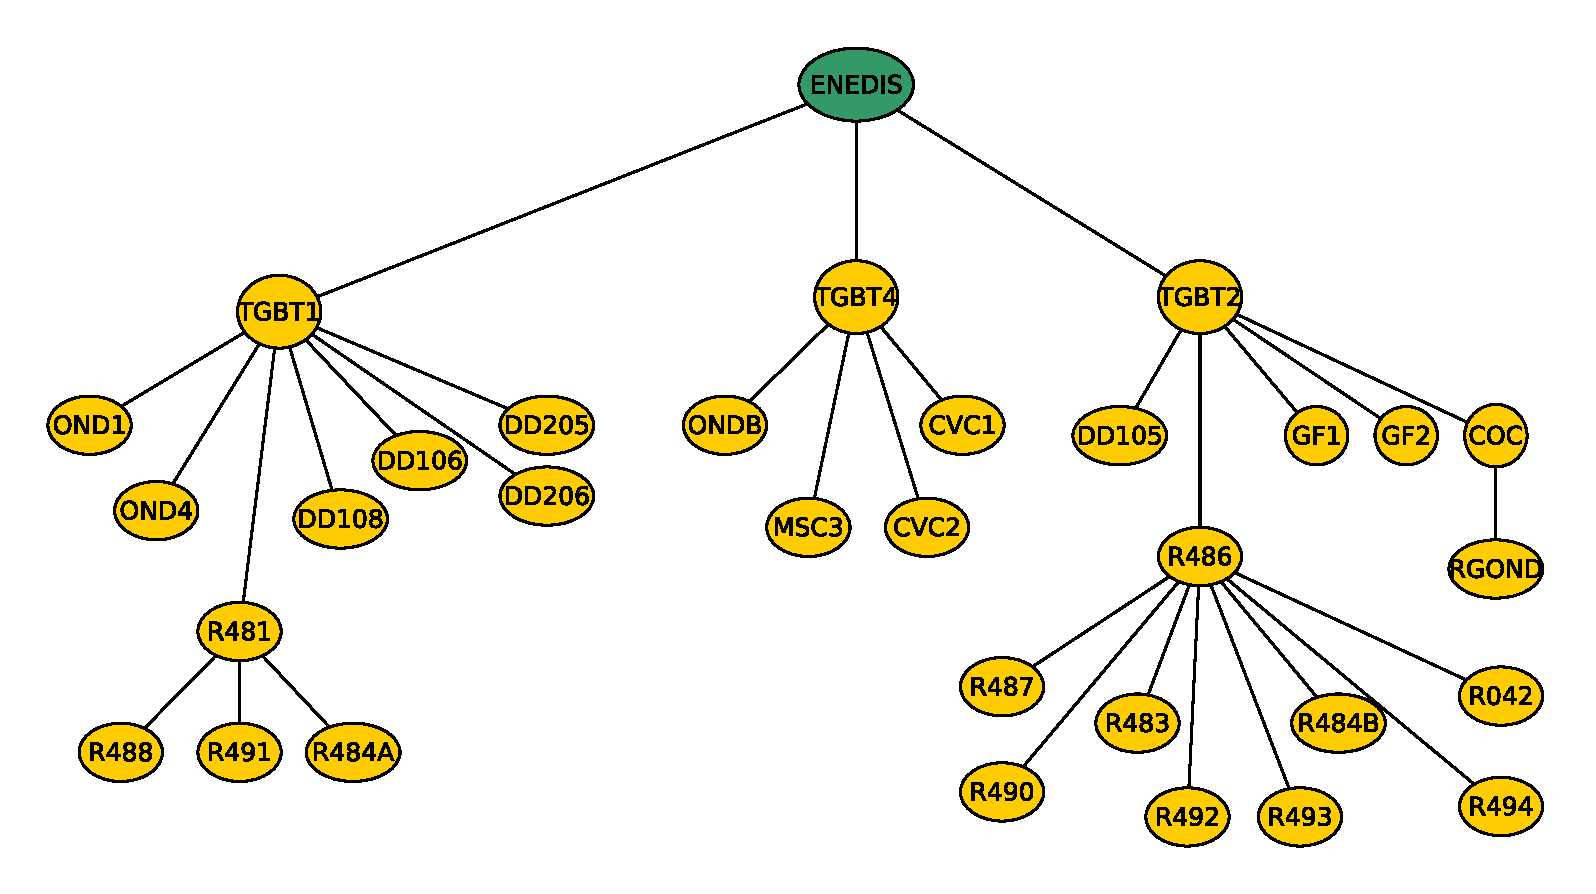
\includegraphics[scale = 0.65]{sousReseauChamplan.eps}
\caption{Le sous-r\'eseau de Champlan \'etudi\'e : Les sources sont {\em TGBT1, TGBT2, TGBT4}. $GF$(1,2) d\'esigne le groupe froid qui g\`ere la climatisation. 
Les tableaux sont {\em DD205, DD206, DD105, DD106, DD108, MSC3, R486, R481, CVC1 et CVC2}. 
Les baies sont {\em R491, R488, R484A, R484B, R042, R483, R487, R492, R490, R493, R494}. Les onduleurs sont indiqu\'es par {\em OND1,OND2,RGOND}. 
Les \'equipements {\em TGBT} sont aliment\'es par une source externe au datacenter, le fournisseur d'\'electricit\'e r\'egional {\em Enedis}.
}
\label{sousReseauChamplan}
\end{figure}
% ---- figure sous-reseau champlan.
\newline

% 3-  coefficients de similarite 
Nous allons calcul\'e la corr\'elation entre les arcs du {\em sous-r\'eseau de Champlan} en supposant que {\em deux arcs incidents \`a un \'equipement sont fortement corr\'el\'es et deux arcs non corr\'el\'es ne poss\`edent aucun \'equipement en commun}.
Chaque arc est identifi\'e par deux \'equipements, celui qui fournit l'\'electricit\'e ($x$) et celui qui en consomme ($y$). Nous d\'esignons par convention $x->y$, l'arc entre $x$ et $y$. Par exemple, l'arc entre $TGBT1$ et $R481$ est not\'e $TGBT1->R481$. 
\newline
Soient trois arcs $x->y$ et $y->z$ et $t->u$. 
Le coefficient de similarit\'e $corr(x->y,y->z) = 1$ signifie que les arcs $x->y$ et $y->z$  ont les m\^emes profils de consommation, partagent le sommet $y$ et sont fortement corr\'el\'es. De m\^eme, le coefficient $corr(x->y,t->u) = 0$ indique que les arcs  $x->y$ et $t->u$ ne sont pas corr\'el\'es c'est-\`a-dire qu'ils n'ont pas de sommet en commun et que leurs profils de consommation sont diff\'erents.
\newline

% ---- figure sous-reseau champlan
\begin{figure}[htb!] 
\centering
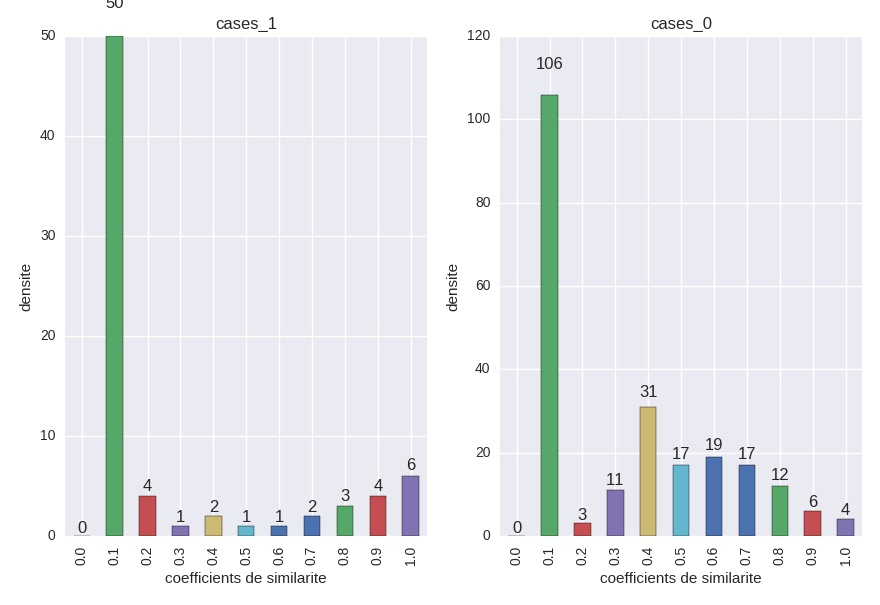
\includegraphics[scale = 0.55]{distribution_0_1_distance_pearson.jpeg}
\caption{Distribution des coefficients des similarit\'es selon les arcs qui sont incidents.
$cases\_1$ d\'esigne les arcs incidents et $cases\_0$ d\'esigne les arcs non incidents dans le {\em sous-r\'eseau de Champlan}.
Le coefficient de similarit\'e $0.1$ indique toutes les valeurs dans l'intervalle $[0.1, 0.2[$.
}
\label{distribution_0_1_distance_pearson}
\end{figure}
% ---- figure sous-reseau champlan.
% 4 erreur de similarite et categorisation de ces erreurs 
Nous disposons de la topologie \'electrique r\'eelle de {\em Champlan}.
Nous comparons  les coefficients de similarit\'e  calcul\'es par rapport aux arcs qui sont incidents dans la topologie de {\em Champlan}.
Pour ce faire, nous pr\'esentons, dans la figure \ref{distribution_0_1_distance_pearson}, les distributions des arcs incidents et non incidentes  en fonction des coefficients de similarit\'e. Les arcs non incidentes sont d\'esign\'es par $cases\_0$ et les arcs incidents par $cases\_1$.
	% arcs non adjacents : prkoi on a des coeff = 1?
		% ---- figure  profils_consommation_cases_0_similarite_1
		\begin{figure}[htb!] 
		\centering
		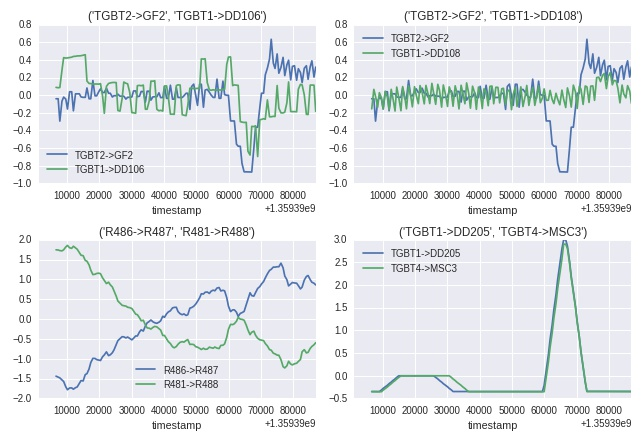
\includegraphics[scale = 0.65]{profils_consommation_cases_0_similarite_1.jpeg}
		\caption{ Profils de consommation des paires d'arcs n'ayant aucun \'equipement en commun. 
		En haut \`a gauche, nous avons les courbes des arcs $TGBT2->GF2$, $TGBT1->DD106$. 
		En haut \`a droite, les courbes des arcs $TGBT2->GF2$, $TGBT1->DD108$. 
		En bas \`a gauche, les courbes des arcs $R486->R487$, $R481->R488$.
		En bas \`a droite,  les courbes des arcs  $TGBT1->DD205$, $TGBT4->MSC3$
		}
		\label{profils_consommation_cases_0_similarite_1}
		\end{figure}
%		\FloatBarrier
		% ---- figure  profils_consommation_cases_0_similarite_1
	La distribution des arcs non incidents est asym\'etrique vers la gauche. Cela est normale puisque nous avons suppos\'e que les arcs non incidents ont des coefficients de similarit\'e qui tendent vers $0$. 
	Cependant, nous avons $4$ paires d'arcs qui ont des coefficients $corr(x->y,y->z) = 1$. La figure \ref{profils_consommation_cases_0_similarite_1} pr\'esente les profils de consommation de ces $4$ paires arcs. Nous constatons que :
	\begin{itemize}
		\item Les arcs $R486->R487$ et $R481->R488$ ont des profils oppos\'es et en appliquant la valeur absolue sur les valeurs de chaque s\'erie, les profils se superposent. Il n'y a aucune corr\'elation entre cette paire d'arcs. 
		\item Les arcs $TGBT1->DD205$ et $TGBT4->MSC3$ ont leurs profils qui se superposent et la corr\'elation de Pearson entre ces s\'eries est alors nulle.
		\item Les paires d'arcs $TGBT2->GF2$ et $TGBT1->DD106$ ont des courbes qui ont plusieurs points d'intersection. \`A ces points, le coefficient de similarit\'e est nul et est proche de $0$ au voisinage de ces points. La corr\'elation de Pearson entre ces s\'eries est alors nulle. 
	\end{itemize}
	Cela implique que le coefficient de similarit\'e est \'egal \`a $corr(x->y,y->z) = 1$ entre ces paires d'arcs $x->y,y->z$ par l'\'equation \ref{personDistance} alors que ces arcs n'ont aucun sommet en commun dans le graphe de la figure \ref{sousReseauChamplan}.
	Ces erreurs de corr\'elation sont introduites par la m\'ethode de calcul des coefficients.
	\newline  
	% arcs adjacents : prkoi on a des coeff = 0.1?
		% ---- figure profils_consommation_cases_1_similarite_0.1
		\begin{figure}[htb!] 
		\centering
		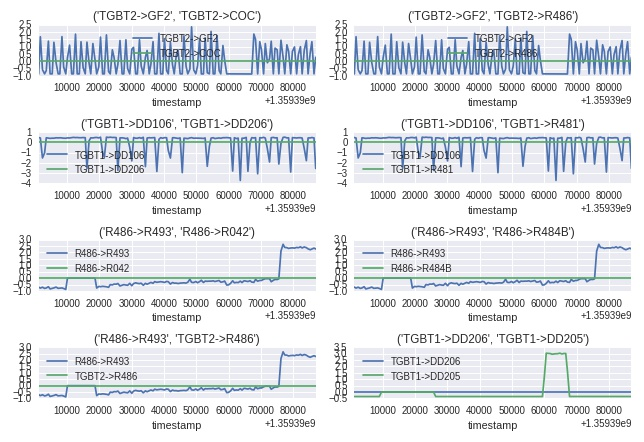
\includegraphics[scale = 0.65]{profils_consommation_cases_1_similarite_01.jpeg}
		\caption{ Profils de consommation des paires d'arcs ayant un \'equipement en commun. 
		les arcs $TGBT2->GF2$ et $TGBT2->COC$ partagent l'\'equipement $TGBT2$.}
		\label{profils_consommation_cases_1_similarite_01}
		\end{figure}
		% ---- figure  profils_consommation_cases_1_similarite_0.1
	En ce qui concerne la distribution des coefficients de similarit\'e des arcs incidents ($cases\_1$), elle est aussi asym\'etrique \`a gauche avec un pic  pour les coefficients appartenant \`a l'intervalle $[0.1,0.2[$. Pour comprendre cette distribution, nous repr\'esentons les profils de consommation de certaines paires d'arcs incidents  ayant leur coefficient de similarit\'e appartenant \`a  l'intervalle $[0.1,0.2[$ dans la figure \ref{profils_consommation_cases_1_similarite_01}.  
	Dans ces repr\'esentations, il y'a toujours une courbe constante et sa pr\'esence est due \`a l'impossibilit\'e de collecter des donn\'ees \`a cause d'une panne. 
	Cette s\'erie contient alors des valeurs nulles. Il y'a aussi la fourniture d'\'energie dans les branches. En effet, la source ne fournit que la quantit\'e d'\'energie demand\'ee par un \'equipement. Les s\'eries des arcs sont diff\'erentes et la distance de Pearson est la plus faible ($corr(x->y,y->z) = 0.1$). 
	Dans ce cas, les erreurs sont introduites par les donn\'ees et le fonctionnement du r\'eseau.
\newline	
Dans les cas d'erreurs de similarit\'e \'enonc\'ees plus haut, nous ne pouvons pas les \'eviter  pendant le calcul des coefficients parce que le m\'ecanisme de r\'ecup\'eration des donn\'ees est d\'efaillant et  l'arr\^et de la consommation d'\'electricit\'e d'une branche est masqu\'e par la mise en service de plusieurs serveurs dans une baie appartenant \`a une autre branche.
\newline 

% matrice de correlation et type d erreurs
Les coefficients de similarit\'e sont regroup\'es dans une matrice sym\'etrique  carr\'ee de dimension $N \times N$ avec $N$ le nombre d'arcs dans le {\em sous-r\'eseau de Champlan}.
Les lignes et les colonnes de la matrice sont les arcs du sous-r\'eseau. Chaque case de la matrice contient un coefficient de similarit\'e entre deux arcs. Les cases de la diagonale de la matrice contiennent les coefficients d'un arc avec lui-m\^eme et sont \'egales \`a $0$.  
Cette matrice est appel\'ee {\em matrice de corr\'elation} et se note $M_c$.
Sur cette matrice, diff\'erentes valeurs de seuils $s \in [0,1]$ sont test\'ees dans le but de d\'eterminer la matrice d'adjacence $M_{c,s}$ du {\em sous-r\'eseau de Champlan}. 
Des arcs $x->y$ et $x->z$ dont leur coefficient $corr(x->y, x->z) \ge s$ ont leur case $M_{c,s}[x->y, x->z] = 1$ sinon $M_{c,s}[x->y, x->z] = 0$ si $corr(x->y, x->z) < s$. 
La figure \ref{distrib_relationAdjacence_seuils_distancePerson} pr\'esente les distributions des relations d'incidences entre les arcs apr\`es l'application  des seuils sur la matrice de corr\'elation. Pour un seuil donn\'e, les relations d'incidences sont regroup\'ees en $4$ cat\'egories :
\begin{itemize}
	\item Les incidences {\em vrais positives} : il existe un sommet en commun entre les arcs et la case associ\'ee de la paire d'arcs $[x->y, x->z]$ est $M_{c,s}(x->y, x->z) = 1$. 
	\item Les incidences {\em vrais n\'egatives} : il existe aucun sommet en commun entre les arcs et la case associ\'ee de la paire d'arcs $[x->y, x->z]$ est $M_{c,s}(x->y, x->z) = 0$. 
	\item Les incidences {\em fausses positives} :  il existe aucun sommet en commun entre les arcs et la case associ\'ee de la paire d'arcs $[x->y, x->z]$ est $M_{c,s}(x->y, x->z) = 1$. 
	\item Les incidences {\em fausses n\'egatives} :  il existe un sommet en commun entre les arcs et la case associ\'ee de la paire d'arcs $[x->y, x->z]$ est $M_{c,s}(x->y, x->z) = 0$. 
\end{itemize}
Les incidences {\em fausses positives} et {\em fausses n\'egatives} constituent des {\em erreurs d'incidences} dans la matrice d'adjacence $M_{c,s}$. Nous consid\'erons aussi certaines incidences {\em vrai positives}  et {\em vrais n\'egatives} comme les {\em erreurs d'incidences}.
Chaque graphique affiche les erreurs d'incidences associ\'ees \`a un seuil. Par exemple, dans le graphique {\em VraiPositive\_ErreurAdjacence} de la figure \ref{distrib_relationAdjacence_seuils_distancePerson} nous avons $17$ paires d'arcs partageant un sommet pour un seuil $s=0.4$. De m\^eme, nous avons $57$ paires d'arcs n'ayant aucun sommet en commun pour un seuil $s=0.4$ dans le graphique {\em fauxNegatives\_ErreurAdjacence} de la figure \ref{distrib_relationAdjacence_seuils_distancePerson}. 
Nous observons qu'il n'existe aucun seuil qui 
maximise les nombres d'incidences {\em vrai positives}  et {\em vrai n\'egatives}  et qui
minimise les nombres  d'incidences {\em fausses positives} et {\em fausses n\'egatives}.
Et cela est due \`a l'introduction des erreurs des coefficients de similarit\'e dans la {\em matrice de corr\'elation} $matE$.
		% ---- figure distrib_relationAdjacence_seuils
		\begin{figure}[htb!] 
		\centering
		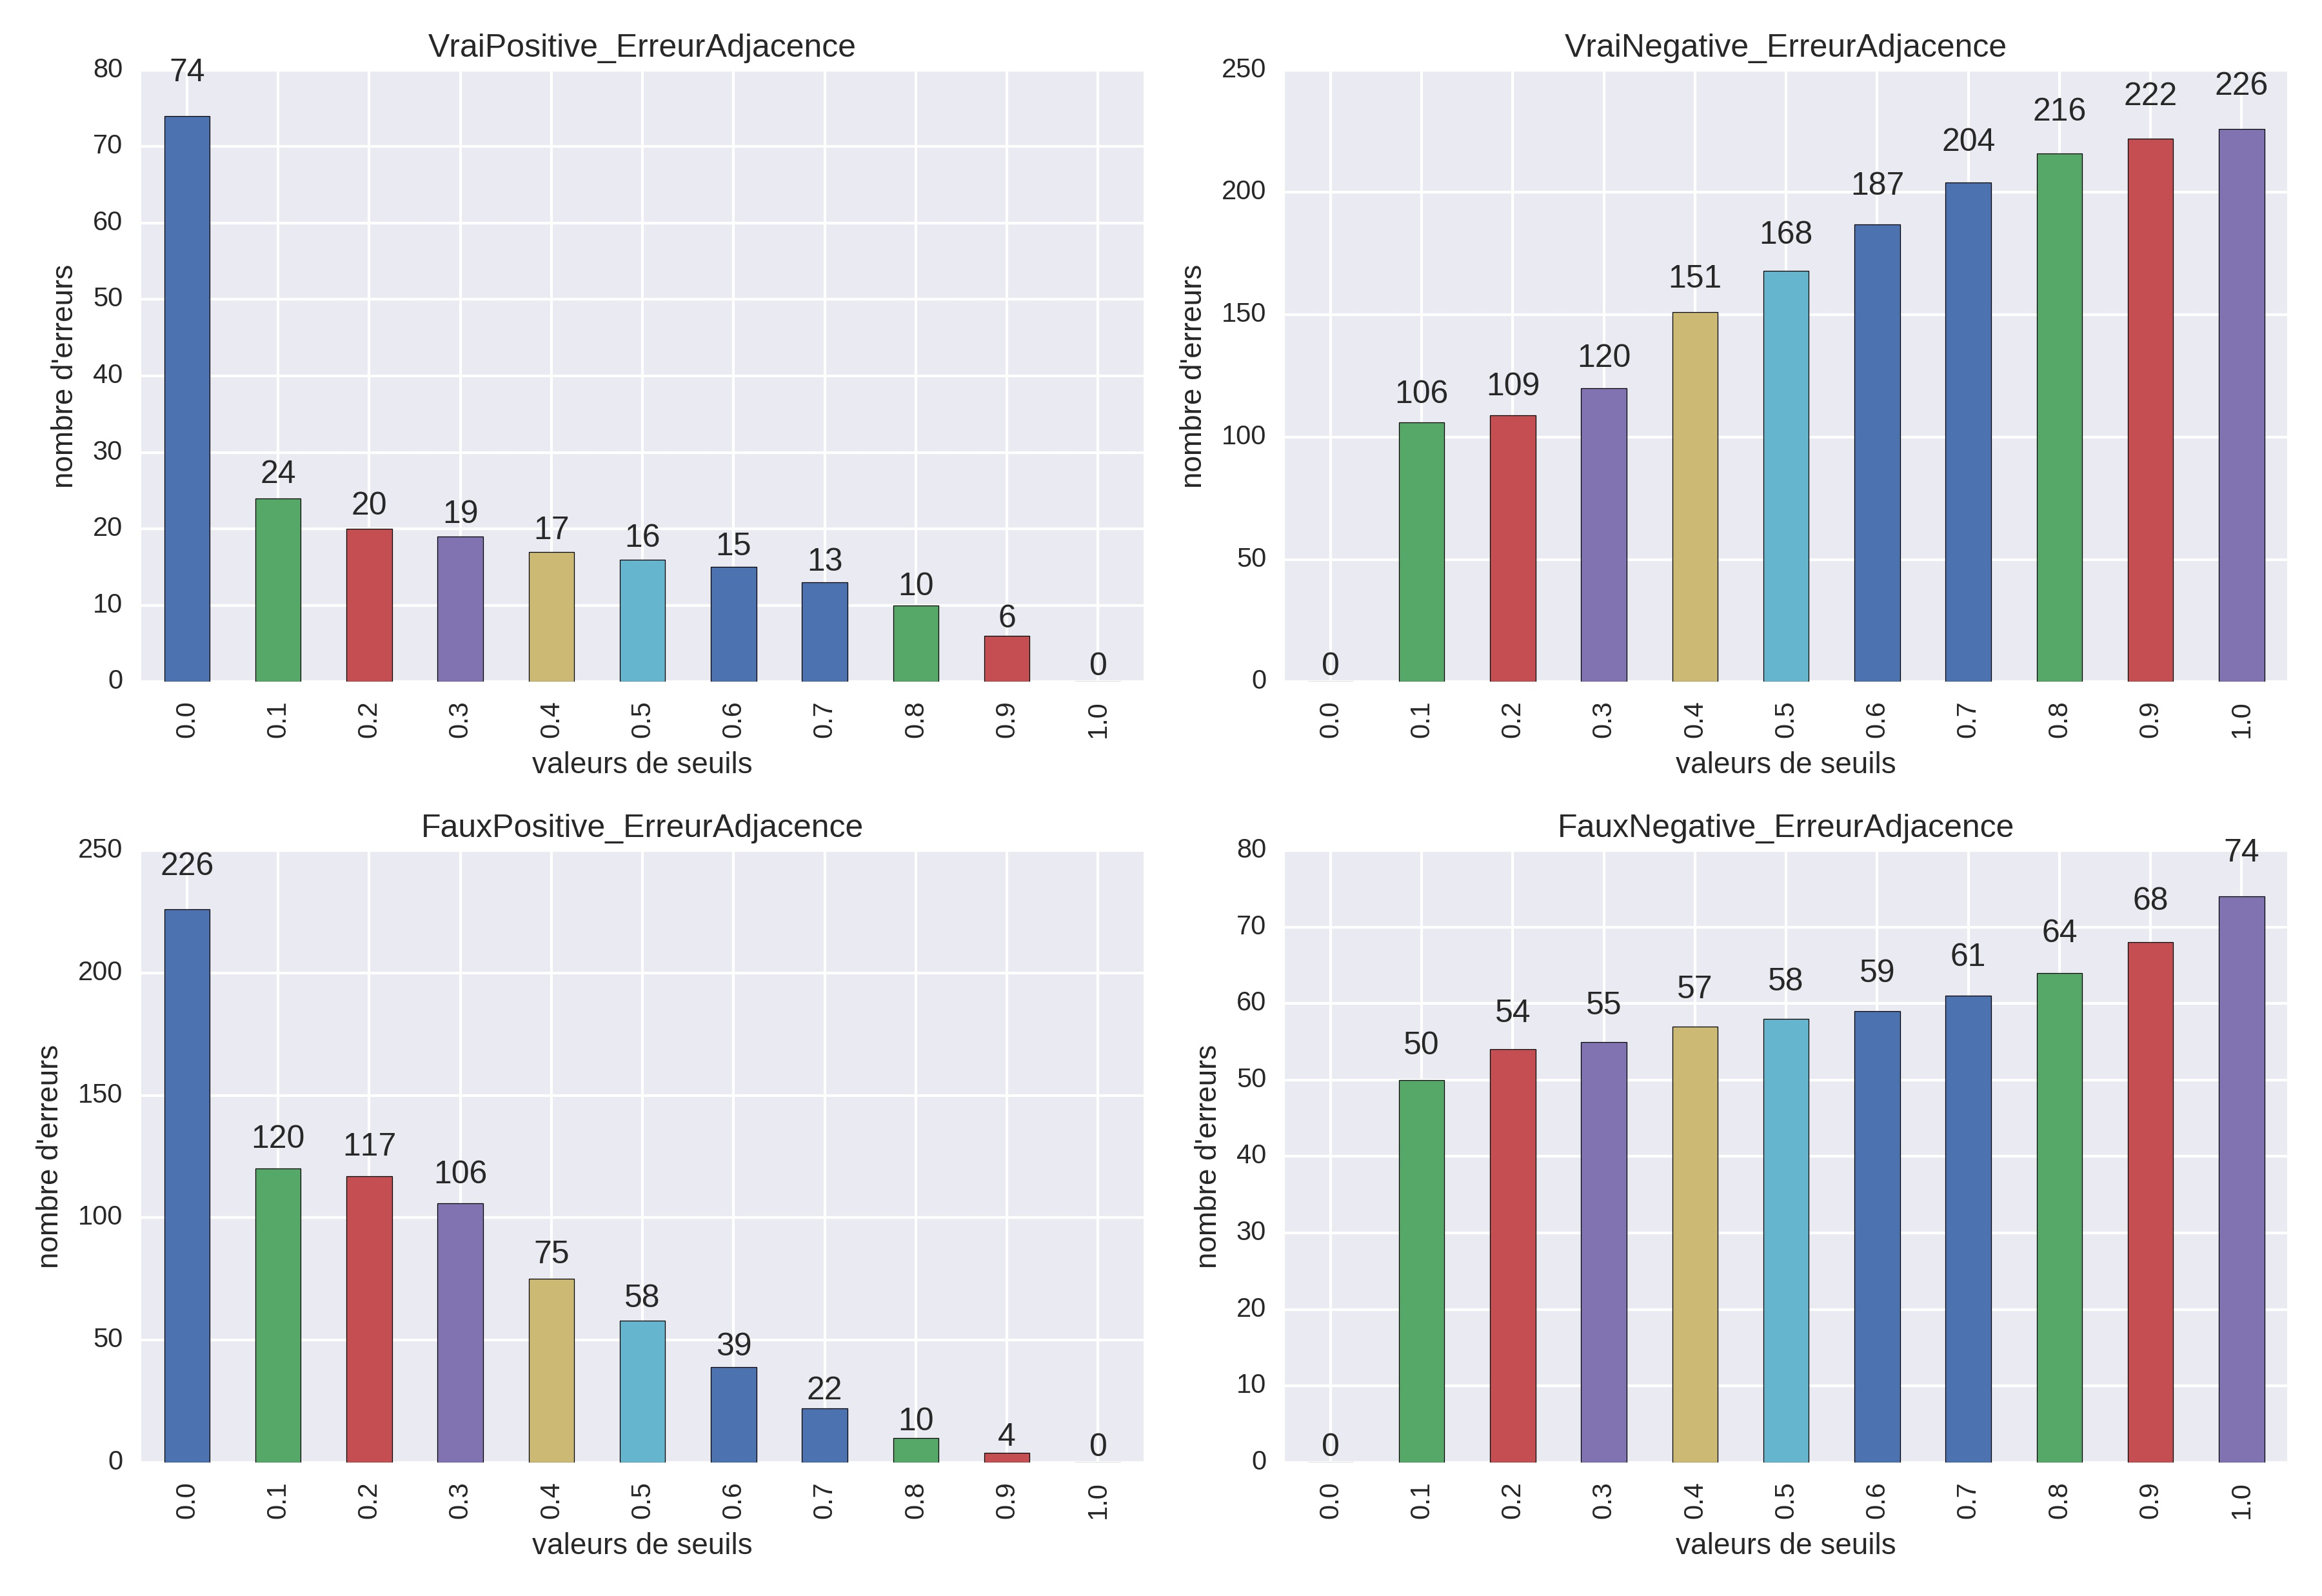
\includegraphics[scale = 0.14]{distrib_relationAdjacence_seuils.jpeg}
		\caption{ Distributions des relations d'incidences entre les arcs apr\`es l'application  de seuils. On distingue $4$ relations d'incidences entre les arcs : incidences {\em fausses positives} (graphique en bas \`a gauche),{\em fausses n\'egatives} (graphique en bas \`a droite), {\em vrais positives} (graphique en haut \`a gauche) et {\em vrai n\'egatives} (graphique en haut \`a droite).
		}
		\label{distrib_relationAdjacence_seuils_distancePerson}
		\end{figure}
		% ---- figure  distrib_relationAdjacence_seuils
\newline

% conclusion
%quel est la grandeur quon a selectionne
%travailler sur un sous graphe de champlan why 
%	presentation de champlan dans le chapitre precedent
%	description du reseau de champlan et presentation du reseau (affichage) 
% calcul des coefficient de similarite
%representation de la matrice de correlation
%comparer les faux positfs avec les faux negatifs 
%choix du seuil ou de epsilon
%conclusion
{\bf Conclusion} :
dans cette section, nous avons limit\'e notre \'etude sur un {\em sous-r\'eseau de Champlan} dans lequel les \'equipements ne sont pas aliment\'es par un onduleur. Ce choix fut pr\'ef\'er\'e \`a cause de notre hypoth\`ese qui stipule que les variations d'\'electricit\'e se propagent dans le r\'eseau. Nous avons calcul\'e les coefficients de similarit\'e $corr$ avec la grandeur {\em P} parce que c'est la seule grandeur qui fournit des mesures en monophas\'e et en triphas\'ee. Certains coefficients de similarit\'e sont \'erron\'es \`a cause des donn\'ees, de la m\'ethode de calcul  et du m\'ecanisme de fonctionnement du r\'eseau de Champlan. Ces coefficients forment la {\em matrice de corr\'elation} $M_c$ carr\'ee et sym\'etrique dans laquelle sont test\'es des seuils. 
Si $M_c$ ne contient aucune erreur de similarit\'e alors il existe un seuil qui d\'etermine la matrice d'adjacence de la topologie du sous-r\'eseau de Champlan. Malheureusement, nous ne sommes pas parvenus \`a d\'eterminer la bonne valeur de seuil et aussi \`a obtenir les coefficients de similarit\'e qui refl\`etent les relations d'adjacences des arcs.


\section{Conclusion du chapitre \ref{timeSeries}}
	Ce chapitre se subdivise en quatres parties.
La premi\`ere partie pr\'esente les domaines dans lesquels l'analyse des s\'eries temporelles est importante. Ensuite, nous exposons notre probl\`eme qui consiste \`a comparer deux s\'eries temporelles en supposant que les variations dans une s\'erie sont reproduites dans l'autre s\'erie.
Pour r\'esoudre notre probl\`eme, nous d\'ecidons de nous servir des m\'ethodes de classification de s\'eries temporelles.
Dans la seconde partie, nous d\'etaillons les m\'ethodes qui se regroupent en trois cat\'egories :
{\em similarit\'e sur les s\'eries enti\`eres, similarit\'e sur les parties significatives, similarit\'e par aggr\'egation des caract\'eristiques descriptives}. Chaque cat\'egorie d\'ecrit des distances de similarit\'e. 
Les avantages et les inconv\'enents de chaque cat\'egorie sont d\'ecrites dans la troisi\`eme partie. Ainsi, en analysant nos donn\'ees et en se basant sur notre hypoth\`ese, nous avons montr\'e que  les m\'ethodes sur les s\'eries enti\`eres sont adapt\'ees \`a notre probl\`eme.
En effet, notre hypoth\`ese stipule que deux arcs partageant un \'equipement ont les m\^emes profils de consommation et leur coefficient de similarit\'e est proche de $1$. Dans le cas contraire,  leur coefficient de similarit\'e tend vers $0$ et les profils de consommation ont des courbes diff\'erentes.
Nous avons alors choisi la {\em distance de Pearson} comme la m\'ethode de similarit\'e parce qu'elle est une m\'etrique, de complexit\'e lin\'eaire, ne traite pas le d\'ecalage temporel et enfin retourne des valeurs appartenant \`a l'intervalle $[0,1]$.
Nous avons appliqu\'e cette distance sur un {\em sous-r\'eseau du datacenter Champlan} parce que ce sous-r\'eseau ne poss\`ede aucun \'equipement aliment\'e par un onduleur.
Ensuite, la seule grandeur qui contient des valeurs en monophas\'e et triphas\'e est la grandeur $P$.
Les coefficients de similarit\'e entre les arcs obtenus avec la grandeur $P$ contiennent des erreurs de similarit\'e. Une erreur de similarit\'e est un coefficient proche de $1$ alors que les arcs ne concourent pas en un \'equipement et vice-versa.
Ces coefficients forment la {\em matrice de corr\'elation} qui appliqu\'ee \`a un seuil propose la matrice d'adjacence du sous-r\'eseau de champlan. Ceci est v\'erifi\'e \`a condition que les coefficients ne contiennent aucune erreur.
Enfin, nous avons montr\'e qu'il est difficile de d\'eterminer la bonne valeur de seuil en pr\'esence des coefficients de similarit\'e \'erron\'es.		

